\documentclass[11pt,a4paper,oneside,openright]{book}
\usepackage[spanish,activeacute,es-noshorthands]{babel}
\usepackage[utf8]{inputenc}
\usepackage[T1]{fontenc}
\usepackage{lmodern}
\usepackage{amsmath, amssymb, amsthm}
\usepackage{graphicx}
\graphicspath{{figuras/m12/}{figuras/}}
\usepackage[dvipsnames]{xcolor}
\usepackage{listings}
\usepackage{geometry}
\geometry{margin=2.5cm, headheight=14pt}
\usepackage{microtype}
\usepackage{booktabs}
\usepackage{longtable}
\usepackage{enumitem}
\usepackage{fancyhdr}
\usepackage{tcolorbox}
\tcbuselibrary{skins, breakable}
\usepackage{caption}
\captionsetup{font=small, labelfont=bf}
\usepackage{hyperref}
\hypersetup{
  colorlinks=true, linkcolor=NavyBlue, citecolor=ForestGreen, urlcolor=BrickRed,
  pdftitle={M12 --- Maquinas de estado del CubeSat INTISAT},
  pdfauthor={INTISAT --- Documentacion tecnica}
}

% ========== Estilo de cajas ==========
\definecolor{cbox-intui}{HTML}{2C5282}
\definecolor{cbox-intui-bg}{HTML}{EBF8FF}
\definecolor{cbox-warn}{HTML}{C53030}
\definecolor{cbox-warn-bg}{HTML}{FFF5F5}
\definecolor{cbox-ok}{HTML}{2F855A}
\definecolor{cbox-ok-bg}{HTML}{F0FFF4}
\definecolor{cbox-tech}{HTML}{B7791F}
\definecolor{cbox-tech-bg}{HTML}{FFFBEB}
\definecolor{cbox-payload}{HTML}{6B46C1}
\definecolor{cbox-payload-bg}{HTML}{FAF5FF}

\newtcolorbox{intui}{
  colback=cbox-intui-bg, colframe=cbox-intui, sharp corners=northwest,
  arc=2pt, boxrule=1pt, fonttitle=\bfseries,
  title=Intuicion, breakable
}
\newtcolorbox{cuidado}{
  colback=cbox-warn-bg, colframe=cbox-warn, sharp corners=northwest,
  arc=2pt, boxrule=1pt, fonttitle=\bfseries,
  title=Cuidado, breakable
}
\newtcolorbox{logrado}{
  colback=cbox-ok-bg, colframe=cbox-ok, sharp corners=northwest,
  arc=2pt, boxrule=1pt, fonttitle=\bfseries,
  title=Ya implementado en INTISAT, breakable
}
\newtcolorbox{tecnico}{
  colback=cbox-tech-bg, colframe=cbox-tech, sharp corners=northwest,
  arc=2pt, boxrule=1pt, fonttitle=\bfseries,
  title=Detalle tecnico, breakable
}
\newtcolorbox{payloadbox}{
  colback=cbox-payload-bg, colframe=cbox-payload, sharp corners=northwest,
  arc=2pt, boxrule=1pt, fonttitle=\bfseries,
  title=El caso INTISAT, breakable
}

% ========== listings ==========
\definecolor{codebg}{HTML}{F8F9FA}
\lstdefinestyle{py}{
  basicstyle=\ttfamily\footnotesize,
  backgroundcolor=\color{codebg},
  keywordstyle=\color{NavyBlue}\bfseries,
  commentstyle=\color{ForestGreen}\itshape,
  stringstyle=\color{BrickRed},
  numbers=left, numberstyle=\tiny\color{gray},
  frame=single, framerule=0.4pt, rulecolor=\color{gray},
  breaklines=true, captionpos=b, language=Python,
  showstringspaces=false, tabsize=2,
}

\pagestyle{fancy}
\fancyhf{}
\renewcommand{\headrulewidth}{0.4pt}
\fancyhead[L]{\small M12 --- Maquinas de estado del INTISAT}
\fancyhead[R]{\small \leftmark}
\fancyfoot[C]{\thepage}
\renewcommand{\chaptermark}[1]{\markboth{#1}{}}

\title{\Huge\bfseries M12 --- Maquinas de estado del CubeSat INTISAT\\[0.5em]
  \large Mision, subsistemas y matriz operacional\\
  \normalsize Documentacion tecnica profunda con diagramas verificados}
\author{Equipo INTISAT}
\date{Mayo 2026}

\begin{document}

\frontmatter
\maketitle

\chapter*{Prefacio}

Este manual es la version impresa, profunda y autocontenida del archivo
HTML \texttt{state\_machines\_cubesat.html}. Es el documento que vas
a llevar a la reunion donde se definen los modos de operacion del
INTISAT con los lideres de cada subsistema.

\textbf{Por que existe este manual.} Un CubeSat NO se opera con
``codigo plano''. Se opera con \emph{maquinas de estado}: un conjunto
de modos discretos, con transiciones bien definidas, donde
\emph{en cualquier instante} el operador de tierra sabe exactamente
en que estado esta el satelite y que comandos puede aceptar. Esto es
diferente al desarrollo de software de aplicacion en Tierra y es una
de las cosas que mas confunde a equipos que vienen de DevOps o de
sistemas empresariales.

\textbf{Que es nuevo respecto al HTML.} Tres cosas:

\begin{enumerate}[leftmargin=2em]
  \item \textbf{Diagramas regenerados en matplotlib} con
    posicionamiento explicito (no Mermaid auto-layout). Cada caja
    esta donde la pusimos, las flechas curvas tienen radios elegidos
    a mano, los colores son semanticos.
  \item \textbf{Significado de cada estado} explicado en parrafos
    completos. El HTML era para presentar; este manual es para
    \emph{entender}.
  \item \textbf{Anclaje al codigo real del INTISAT.} Cuando una FSM
    ya existe en el repositorio, lo marcamos. Cuando todavia es
    propuesta, tambien.
\end{enumerate}

\textbf{Como leerlo.} Lo podes leer secuencialmente (capitulos 1--3
te dan el marco; 4--9 cada subsistema; 10 el roadmap) o usarlo de
referencia abriendo solo el capitulo del subsistema que te toca.

\tableofcontents

\mainmatter

% ============================================================================
\chapter{Que es una maquina de estados y por que importa}
% ============================================================================

\section{La definicion formal y la version honesta}

Una \textbf{maquina de estados finitos} (FSM, \emph{Finite State
Machine}) es una tupla $(S, \Sigma, \delta, s_0, F)$ donde:

\begin{itemize}[leftmargin=2em]
  \item $S$ es un conjunto finito de \emph{estados}.
  \item $\Sigma$ es un conjunto finito de \emph{eventos} (triggers).
  \item $\delta: S \times \Sigma \to S$ es la funcion de transicion.
  \item $s_0 \in S$ es el estado inicial.
  \item $F \subseteq S$ son estados terminales (opcional).
\end{itemize}

Esta es la version del libro de teoria de computacion. La version
honesta, para alguien que esta programando un satelite, es:

\begin{intui}
Una FSM te obliga a escribir, ANTES de codear, una lista de:
\begin{enumerate}[leftmargin=2em]
  \item Todos los modos en los que puede estar mi sistema.
  \item Que eventos pueden hacer que cambie de modo.
  \item Cual es la transicion exacta para cada par (modo, evento).
\end{enumerate}
Si no podes responder estas 3 preguntas, no sabes que hace tu sistema
realmente. Y si no lo sabes en Tierra, vas a tener un satelite que
hace cosas que no entendes en orbita.
\end{intui}

\section{Por que los CubeSats no usan codigo plano}

En un servidor web, si el codigo hace algo raro, te conectas por SSH,
mirás los logs, corrés un \texttt{strace} y arreglás. En un CubeSat
no podes hacer nada de eso. Tenes:

\begin{itemize}[leftmargin=2em]
  \item \textbf{Ventanas de comunicacion} de 5--10 minutos por orbita,
    cada $\sim$90 min.
  \item \textbf{Ancho de banda} que va de 1.2 kbps (UHF) a 100 kbps
    (S-Band en el mejor caso).
  \item \textbf{Sin acceso fisico.} Si algo se bloqueo, esperas el
    proximo watchdog reset (puede ser horas).
  \item \textbf{Decisiones autonomas.} El satelite tiene que poder
    decidir solo cuando entrar en SAFE, cuando hacer downlink, cuando
    apagar el payload.
\end{itemize}

\begin{cuidado}
Si tu codigo del satelite tiene 50 variables booleanas tipo
\texttt{is\_charging}, \texttt{is\_pointing}, \texttt{can\_transmit},
\texttt{has\_data\_ready}\ldots tenes una FSM \emph{implicita}
con $2^{50}$ estados posibles. La mayoria de esos estados son
invalidos o catastroficos, pero no podes razonar sobre ellos. \\

Hacer la FSM explicita con $\sim$10 estados bien definidos no es
``hacer mas trabajo''; es \emph{descubrir} cuales de los $2^{50}$
estados realmente queres que existan.
\end{cuidado}

\section{La gran intuicion: en cualquier momento, un solo estado}

La regla de oro de una FSM es: \textbf{en cualquier instante, el
sistema esta en EXACTAMENTE un estado.} No dos. No medio. Uno.

Esto suena trivial pero es lo mas duro de respetar cuando uno
arranca. La tentacion natural es decir ``bueno, estoy cargando la
bateria \emph{y} apuntando al sol \emph{y} esperando un comando''.
La FSM te obliga a decir: ``estoy en NOMINAL, lo cual implica que
estoy cargando, apuntando y esperando, pero el unico estado es
NOMINAL''.

Esa disciplina convierte un sistema que ``a veces no funciona y no
sabemos por que'' en un sistema donde podes preguntar ``en que estado
estabas?'' y la respuesta es univoca.

% ============================================================================
\chapter{Los 3 niveles de jerarquia}
% ============================================================================

Un CubeSat no es \emph{una} maquina de estados. Es una jerarquia
de tres niveles. Confundirlos es el error mas comun.

\begin{figure}[h]
\centering
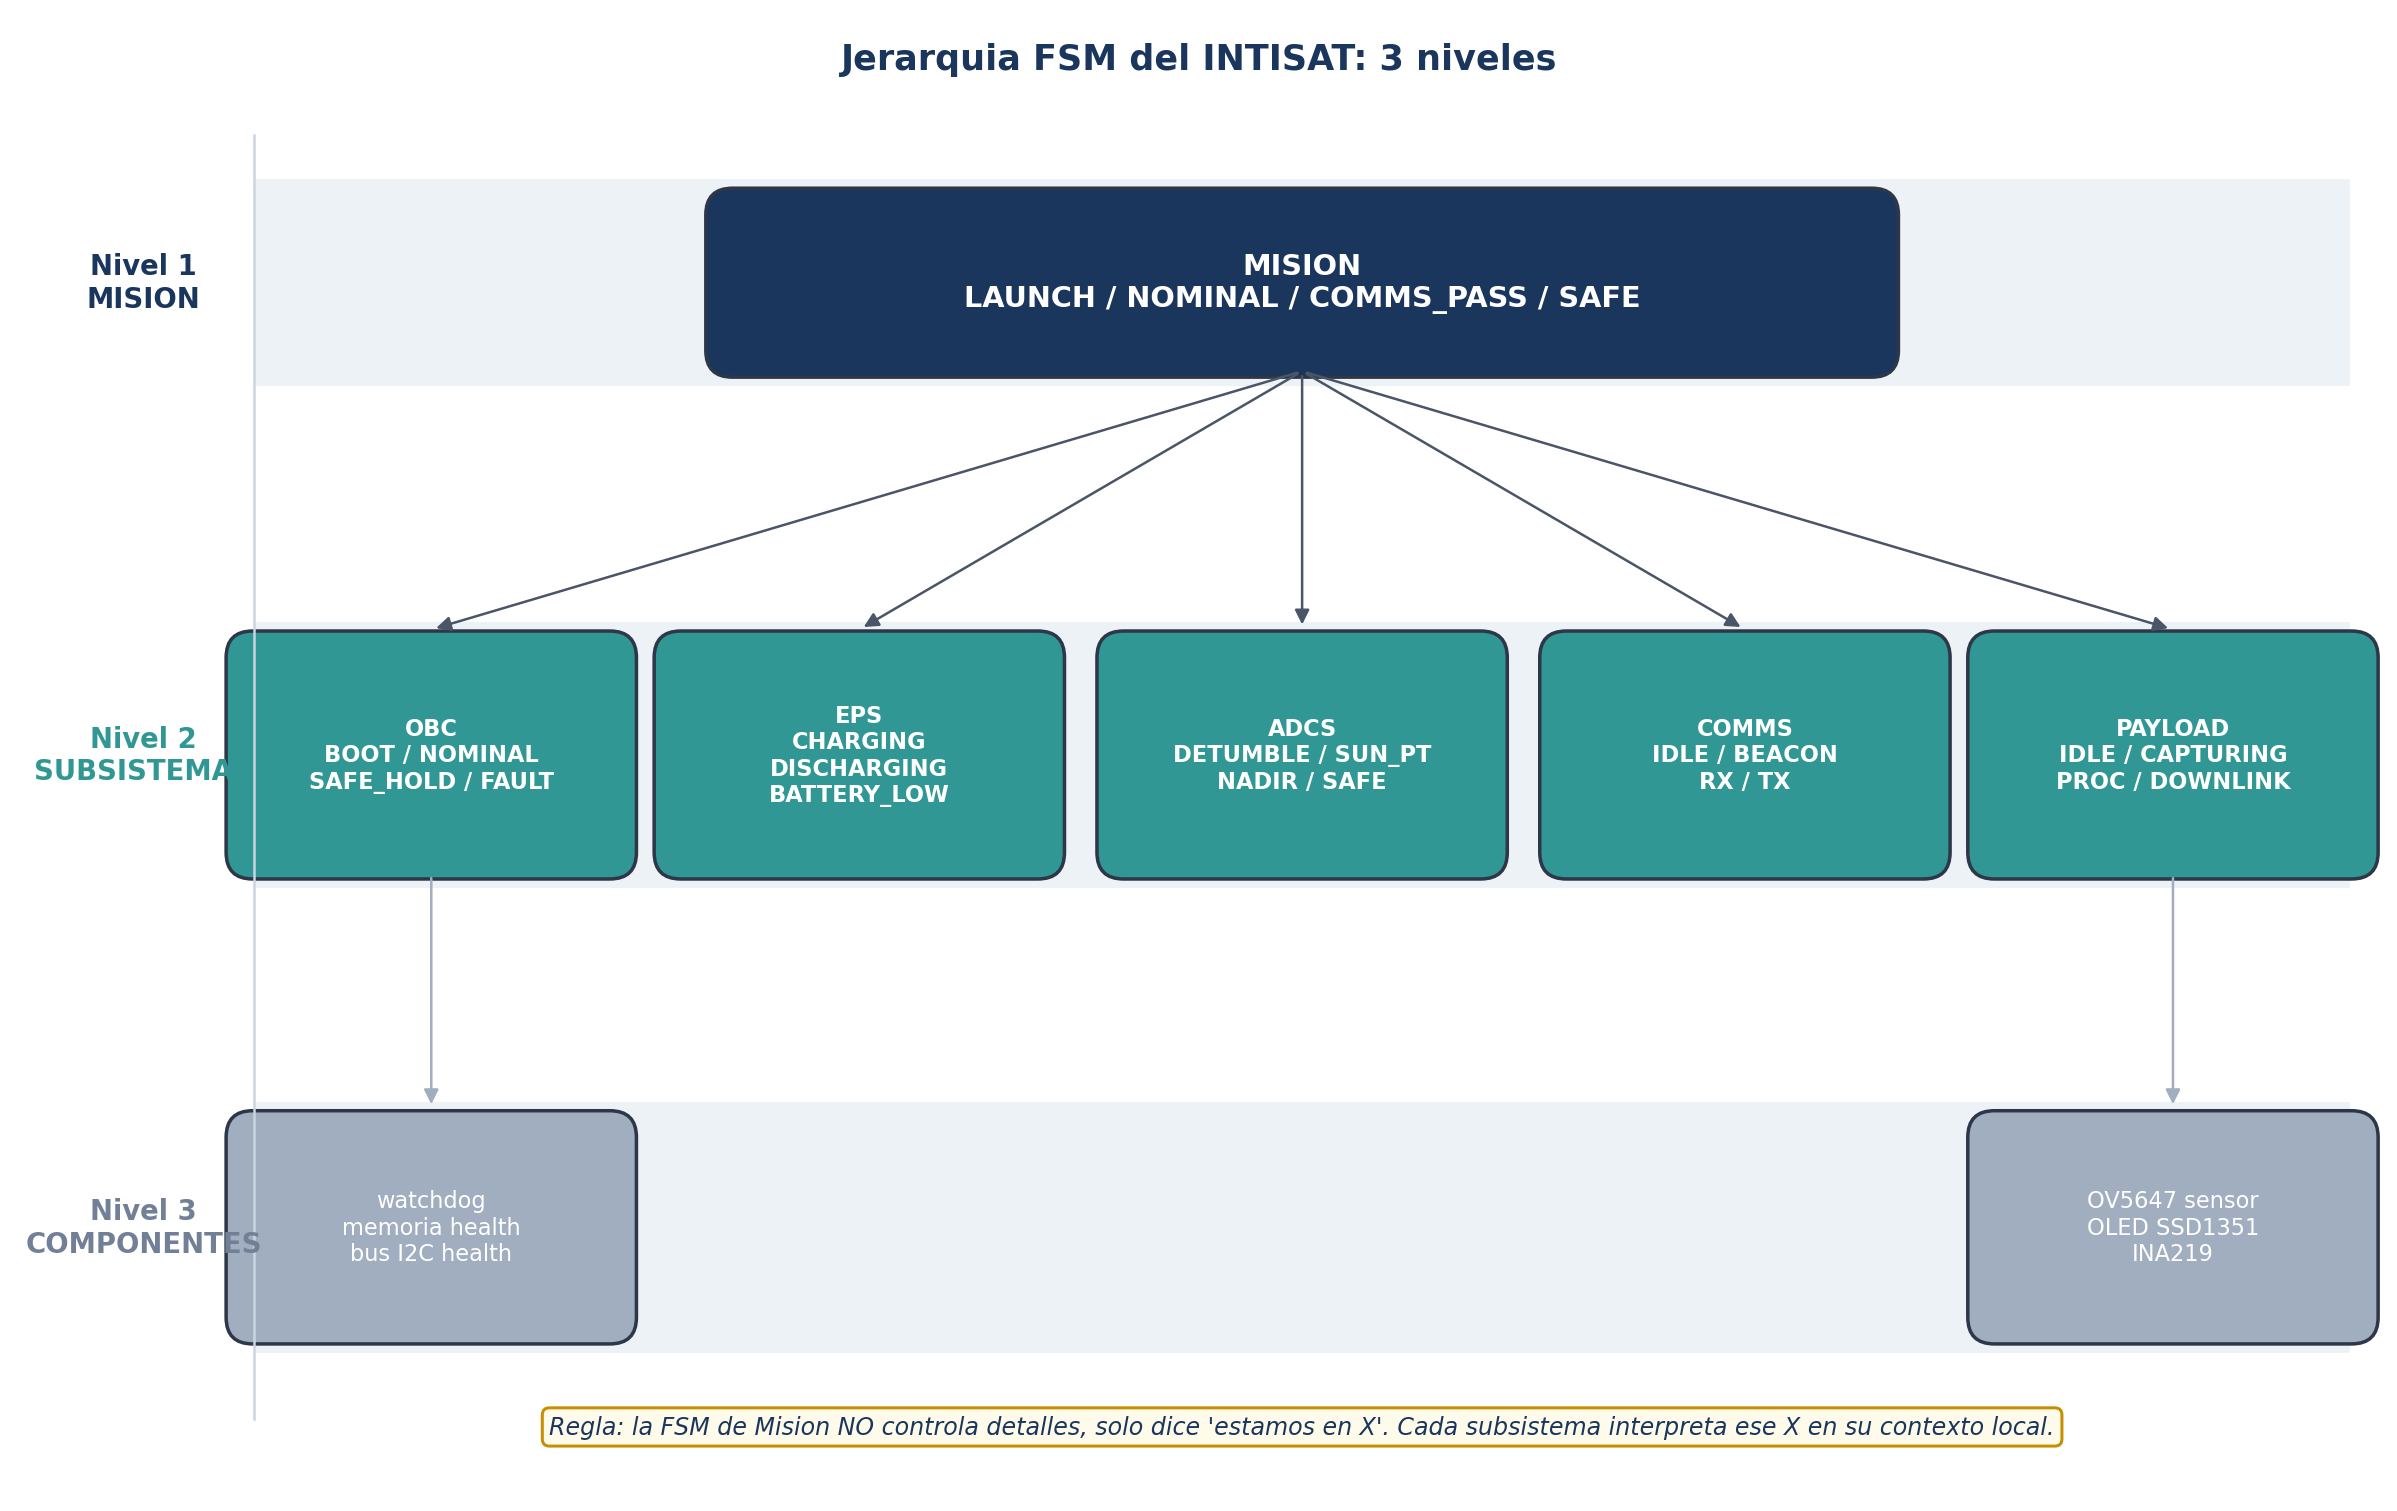
\includegraphics[width=\linewidth]{fig01_jerarquia.png}
\caption{Jerarquia de FSMs en el INTISAT. La FSM de mision (nivel 1) no
controla detalles; cada subsistema (nivel 2) tiene su propia FSM, e
internamente cada componente (nivel 3) tambien.}
\end{figure}

\section{Nivel 1 --- la FSM de MISION}

Es lo que ve el operador de tierra. Son 8 modos a alto nivel: LAUNCH,
DETUMBLE, COMMISSIONING, NOMINAL, PAYLOAD\_OP, COMMS\_PASS, ECLIPSE,
SAFE, EOL. La FSM de mision \textbf{NO} mira los pines del CM5, no
sabe que el OLED esta encendido, no sabe el voltaje del shunt. Solo
sabe: ``estamos en NOMINAL'' o ``estamos en SAFE''.

\section{Nivel 2 --- la FSM de cada SUBSISTEMA}

Cada subsistema (OBC, EPS, ADCS, COMMS, PAYLOAD) tiene su propia FSM
con sus propios estados internos. Cuando la mision esta en NOMINAL,
cada subsistema interpreta ``NOMINAL'' en su contexto local:

\begin{itemize}[leftmargin=2em]
  \item EPS en NOMINAL = ``estoy CHARGING''.
  \item ADCS en NOMINAL = ``estoy en SUN\_POINTING''.
  \item PAYLOAD en NOMINAL = ``estoy en IDLE, listo para CMD\_START\_CAPTURE''.
\end{itemize}

La traduccion entre ``modo de mision'' y ``estado interno de cada
subsistema'' la define la \textbf{matriz modos $\times$ subsistemas}
(capitulo 4).

\section{Nivel 3 --- componentes}

Bajo cada subsistema hay componentes con su propia mini-FSM:

\begin{itemize}[leftmargin=2em]
  \item En el OBC: el watchdog timer, el chequeo de memoria, el bus
    I2C.
  \item En el PAYLOAD: el sensor OV5647 (apagado / configurado /
    capturando), el OLED SSD1351 (apagado / mostrando estado), el
    INA219 (idle / midiendo).
\end{itemize}

\begin{intui}
\textbf{La regla:} cada nivel coordina al de abajo pero no se mete en
detalles. La FSM de mision NO le dice al ADCS ``encende el reaction
wheel X''; le dice ``estamos en PAYLOAD\_OP'' y el ADCS sabe que en
PAYLOAD\_OP tiene que estar en NADIR\_POINTING, y para eso comanda a
sus componentes internos.
\end{intui}

% ============================================================================
\chapter{La FSM de MISION: el satelite completo}
% ============================================================================

\begin{figure}[h]
\centering
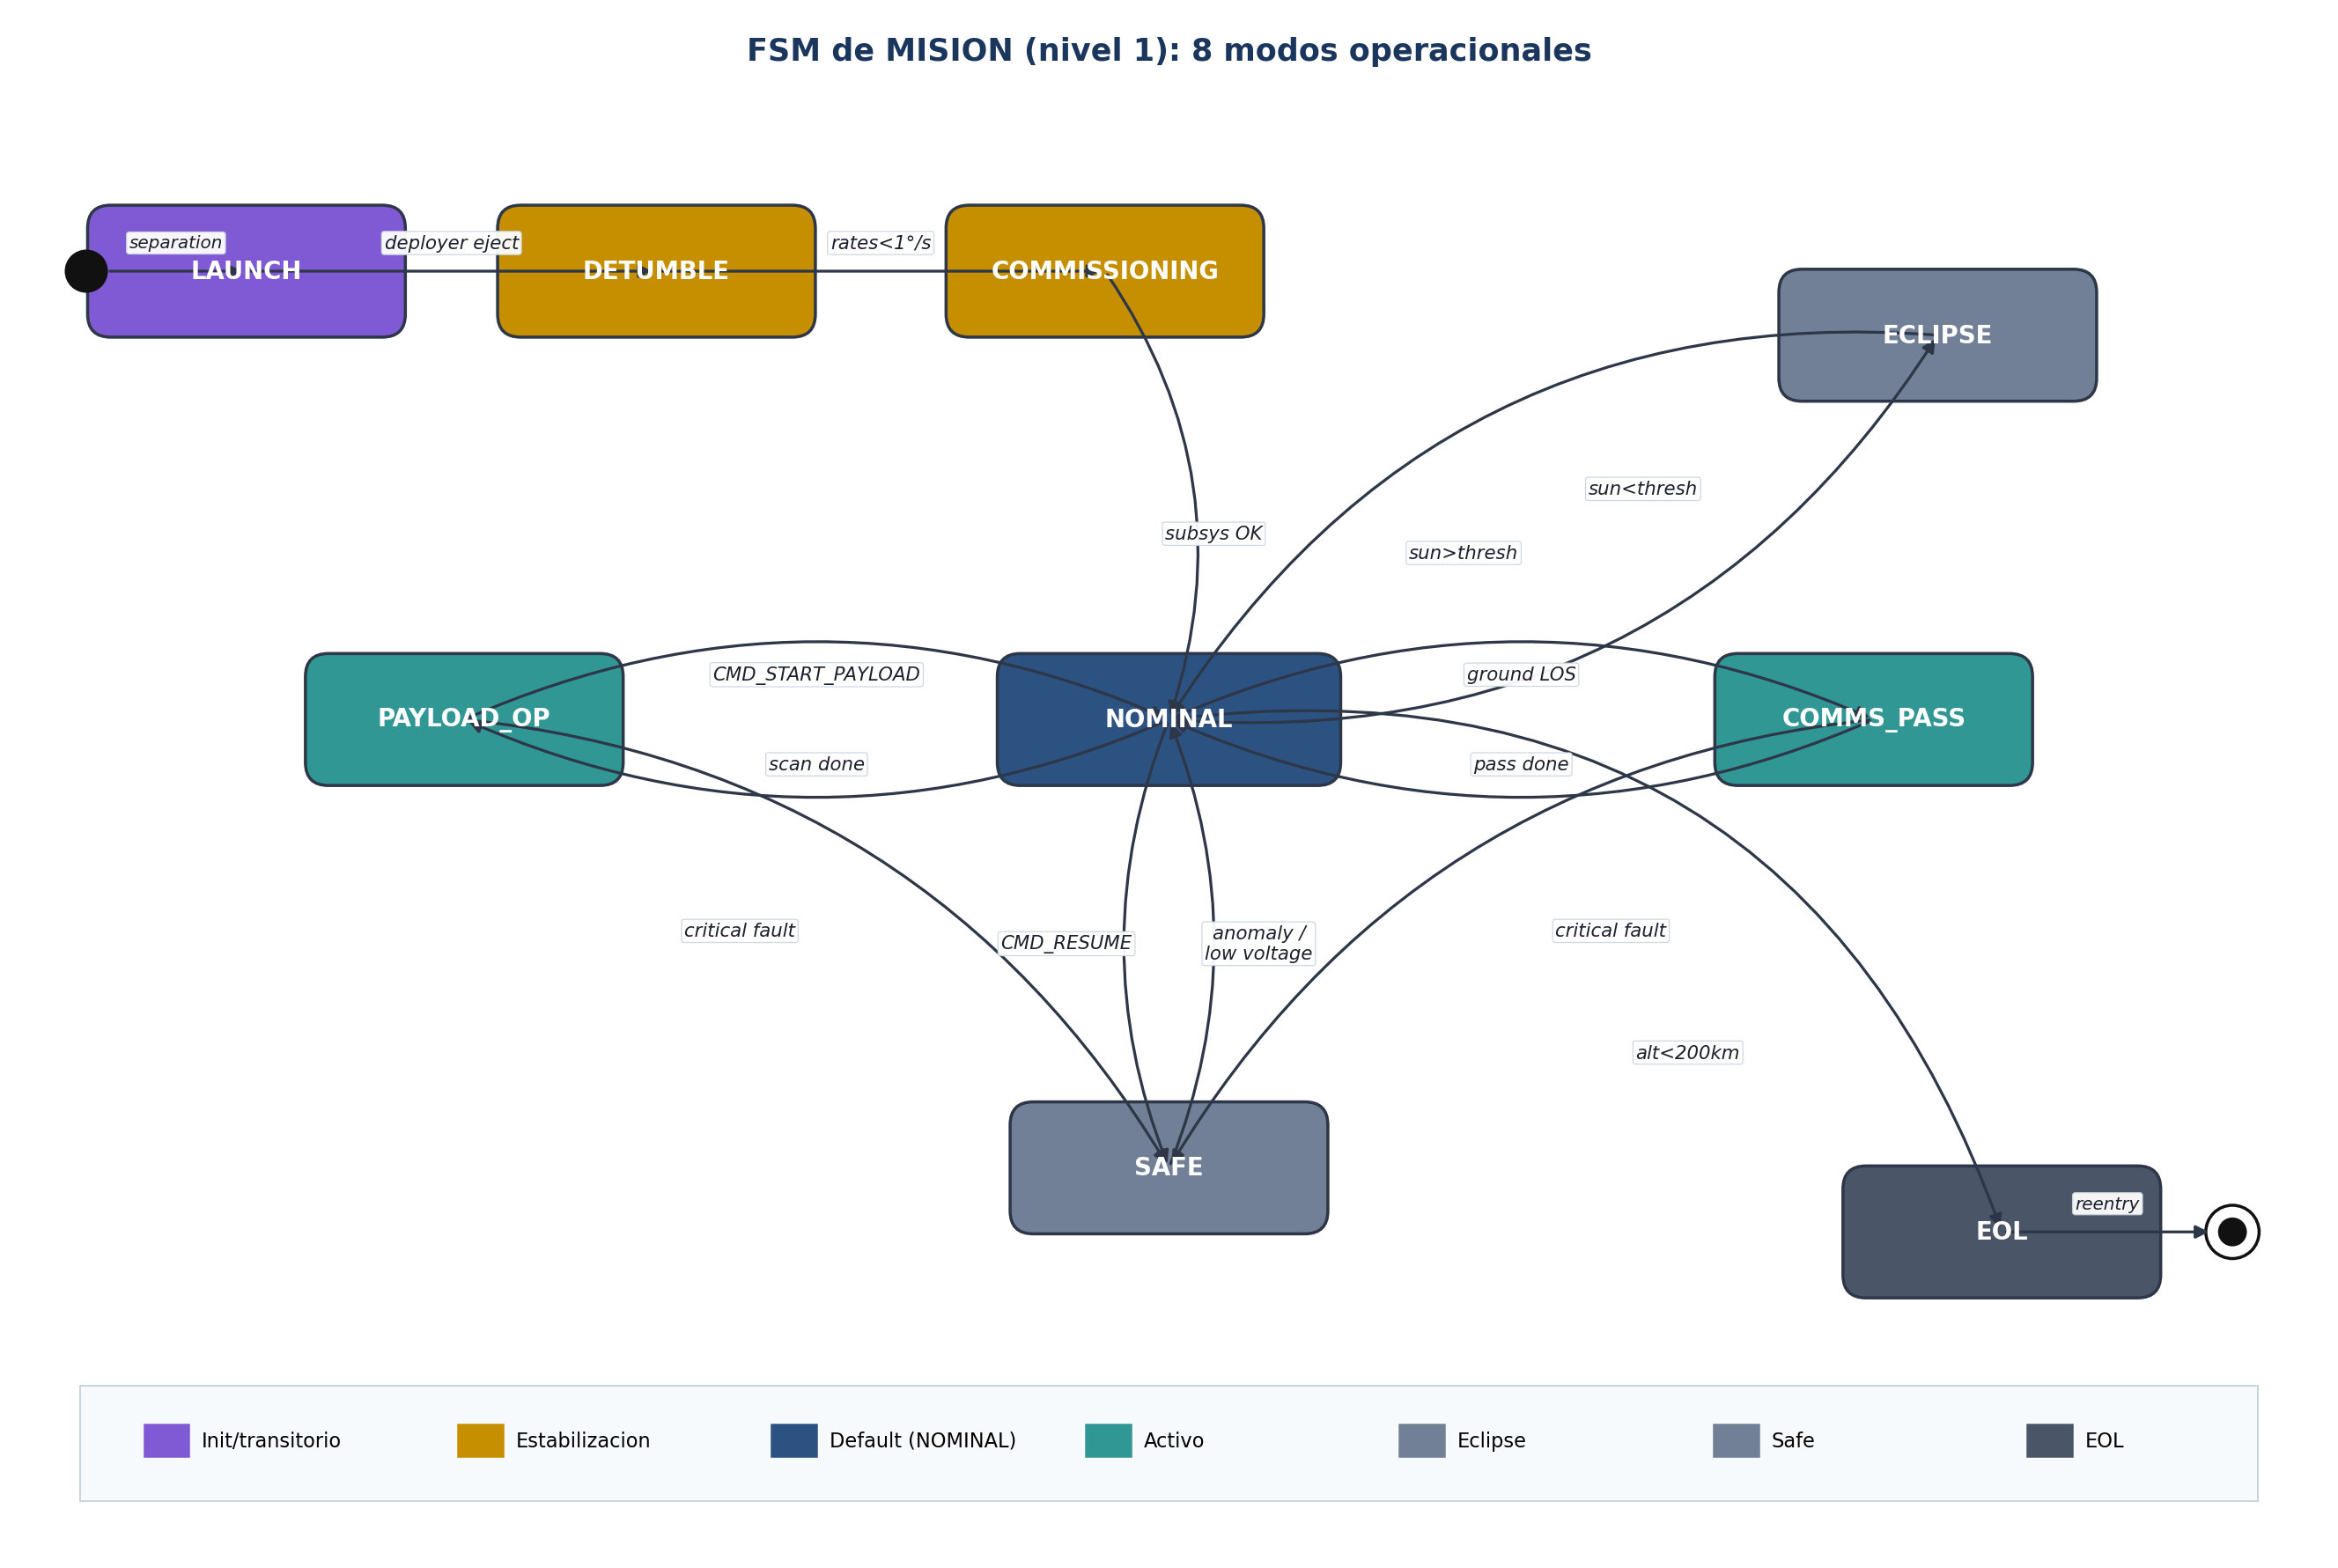
\includegraphics[width=\linewidth]{fig02_mision.png}
\caption{FSM de mision. 8 modos operacionales del INTISAT, con transiciones
desde la separacion del deployer hasta el end-of-life.}
\end{figure}

A continuacion describimos cada uno de los 8 modos. Para cada uno
indicamos: \textbf{(a)} cuando se entra, \textbf{(b)} que hace el
satelite en ese modo, \textbf{(c)} cuando se sale.

\section{LAUNCH --- de la base de lanzamiento al deployer}

\textbf{(a) Entrada:} desde el momento que el satelite esta en el
deployer del cohete hasta unos minutos despues de la eyeccion.
Tipicamente entre T-30 min y T+45 min, donde T es la hora de
lanzamiento.

\textbf{(b) Que hace:} \emph{nada}. Por norma de seguridad de los
deployers (NanoRacks, ISIPOD, etc.), el CubeSat debe estar
ELECTRICAMENTE INERTE hasta que el switch de despliegue se cierra.
Esto implica:

\begin{itemize}[leftmargin=2em]
  \item Bateria conectada pero rails de potencia abiertos.
  \item OBC en estado BOOT (no NOMINAL).
  \item Radio apagado (no se puede transmitir desde dentro del cohete).
  \item ADCS apagado (los actuadores no deben moverse).
\end{itemize}

\textbf{(c) Salida:} cuando el switch de despliegue (RBF + deployment
switches) se cierra. Tipicamente $\sim$30 minutos despues de la
eyeccion, segun ECSS-E-ST-70-11C.

\section{DETUMBLE --- frenar el spin de la eyeccion}

\textbf{(a) Entrada:} inmediatamente despues de LAUNCH.

\textbf{(b) Que hace:} el deployer eyecta el CubeSat con un
\emph{spin residual} de hasta 5--10 \textdegree/s. Hay que frenarlo
para poder hacer cualquier cosa util (apuntar, comunicar, generar
energia). El algoritmo clasico es \emph{B-dot}:

\begin{equation}
\vec{m}_{cmd} = -k \cdot \frac{d\vec{B}}{dt}
\end{equation}

donde $\vec{B}$ es el campo magnetico terrestre medido por el
magnetometro y $\vec{m}_{cmd}$ es el dipolo magnetico comandado a los
magnetorquers. El efecto es disipar energia rotacional sin necesidad
de conocer la actitud absoluta. Lleva entre 6 y 48 horas.

\textbf{(c) Salida:} cuando $\|\vec{\omega}\| < 1$ \textdegree/s en
los 3 ejes (criterio tipico).

\begin{tecnico}
B-dot funciona porque la derivada del campo magnetico en frame body
es proporcional al spin. Es robusto: no requiere knowledge de
actitud, solo magnetometro funcional. Es el algoritmo de
``ultima esperanza'' --- si todo lo demas falla, vuelves a B-dot.
\end{tecnico}

\section{COMMISSIONING --- la primera semana en orbita}

\textbf{(a) Entrada:} cuando termina DETUMBLE.

\textbf{(b) Que hace:} chequeo sistematico de cada subsistema. Esta
fase tipicamente dura entre 1 y 2 semanas (no horas como muchos
piensan). Incluye:

\begin{itemize}[leftmargin=2em]
  \item Verificar que todos los rails de potencia entregan voltaje
    correcto.
  \item Calibrar magnetometro y sensores de sol.
  \item Validar el link RF con la estacion de tierra (downlink + uplink).
  \item Probar cada subsistema en aislamiento, despues en conjunto.
  \item Verificar que la temperatura de los componentes esta en rango.
\end{itemize}

\textbf{(c) Salida:} cuando el equipo de operaciones declara
``commissioning complete''. Es una decision humana.

\section{NOMINAL --- el modo ``default''}

\textbf{(a) Entrada:} terminado COMMISSIONING, o desde COMMS\_PASS /
PAYLOAD\_OP / SAFE.

\textbf{(b) Que hace:} es el modo ``\emph{quiescente}''. El satelite:

\begin{itemize}[leftmargin=2em]
  \item Apunta paneles al sol (ADCS: SUN\_POINTING).
  \item Carga bateria (EPS: CHARGING).
  \item OBC corriendo nominal, escuchando uplink.
  \item Radio en IDLE (RX latente, BEACON cada 30 s).
  \item Payload OFF o IDLE.
\end{itemize}

Es el modo donde el INTISAT pasa $\sim$80\% del tiempo.

\textbf{(c) Salida:} hacia PAYLOAD\_OP (comando), COMMS\_PASS (entra
en LOS con la estacion), ECLIPSE (sol bajo), SAFE (anomalia), EOL
(altitud final).

\section{PAYLOAD\_OP --- el experimento}

\textbf{(a) Entrada:} comando \texttt{CMD\_START\_PAYLOAD} desde
tierra.

\textbf{(b) Que hace:} es el ``why we're here''. Para el INTISAT:

\begin{enumerate}[leftmargin=2em]
  \item ADCS apunta a nadir (NADIR\_POINTING) durante $\sim$10 min.
  \item Payload despierta del IDLE: PAYLOAD: CAPTURING.
  \item Captura 25 frames con OV5647 + mascara lensless.
  \item Procesa con la red neuronal (Real-ESRGAN o similar).
  \item Exporta a almacenamiento.
  \item Vuelve a IDLE y devuelve el bus a NOMINAL.
\end{enumerate}

\textbf{(c) Salida:} scan completo (vuelve a NOMINAL), o fault
critico (va a SAFE).

\begin{logrado}
El payload del INTISAT YA TIENE esta secuencia implementada como FSM
en \texttt{cubesat/commands.py:STATE\_*}. La estudiamos en detalle
en el capitulo 9.
\end{logrado}

\section{COMMS\_PASS --- la ventana de comunicacion}

\textbf{(a) Entrada:} cuando entra LOS (\emph{Line Of Sight}) con la
estacion de tierra. Se predice con TLE (Two-Line Element).

\textbf{(b) Que hace:}

\begin{itemize}[leftmargin=2em]
  \item ADCS apunta antena al ground station (TARGET\_POINTING).
  \item COMMS pasa de IDLE a TX (downlink) o RX (uplink).
  \item Payload puede estar haciendo DOWNLINK si quedo data de scans
    previos.
\end{itemize}

\textbf{(c) Salida:} cuando se pierde LOS. Tipicamente 5--10 min por
pase.

\section{ECLIPSE --- el lado oscuro de la orbita}

\textbf{(a) Entrada:} cuando el sensor de sol detecta $<$5\% del
flujo nominal.

\textbf{(b) Que hace:}

\begin{itemize}[leftmargin=2em]
  \item EPS pasa a DISCHARGING (sin generacion solar).
  \item ADCS pasa a INERTIAL\_HOLD (no hay vector solar para apuntar).
  \item OBC opcionalmente entra en MAINTENANCE (limpieza de logs,
    defrag).
  \item Payload normalmente OFF (a menos que se programe un scan
    nocturno).
\end{itemize}

\textbf{(c) Salida:} cuando vuelve el sol. Tipicamente 35 min en
orbita baja.

\section{SAFE --- el modo de proteccion}

\textbf{(a) Entrada:} CUALQUIER anomalia critica. Ejemplos:

\begin{itemize}[leftmargin=2em]
  \item EPS reporta BATTERY\_CRITICAL.
  \item Watchdog del OBC se dispara 3 veces.
  \item Temperatura fuera de rango.
  \item Comando ground \texttt{CMD\_SAFE} explicito.
\end{itemize}

\textbf{(b) Que hace:} apaga TODO lo no esencial. Solo quedan:

\begin{itemize}[leftmargin=2em]
  \item OBC en SAFE\_HOLD (consumo $\sim$1 W).
  \item COMMS en BEACON (transmite telemetria minima).
  \item ADCS en DETUMBLE (proteccion contra spin).
\end{itemize}

NO acepta comandos no-criticos. Solo \texttt{CMD\_RESUME} y comandos
de telemetria.

\textbf{(c) Salida:} comando \texttt{CMD\_RESUME} desde tierra,
DESPUES de que el equipo de operaciones haya verificado que la causa
de la anomalia esta resuelta.

\begin{cuidado}
SAFE no es ``modo error''. Es ``modo conservador hasta que humanos
decidan''. Un CubeSat puede pasar dias en SAFE sin problema. Salir
de SAFE prematuramente es la causa numero uno de perdida total de
mision.
\end{cuidado}

\section{EOL --- end of life}

\textbf{(a) Entrada:} cuando la altitud cae por debajo de un umbral
(tipicamente 200 km) o cuando la mision se declara terminada por
otra razon.

\textbf{(b) Que hace:} preparacion para reentrada:

\begin{itemize}[leftmargin=2em]
  \item Borrado seguro de datos sensibles.
  \item Beacon final con telemetria de fin de vida.
  \item ADCS off (los magnetorquers no aceleran la reentrada).
\end{itemize}

\textbf{(c) Salida:} la reentrada atmosferica completa la mision.

% ============================================================================
\chapter{La matriz modos x subsistemas (la ``rosetta'')}
% ============================================================================

\begin{figure}[h]
\centering
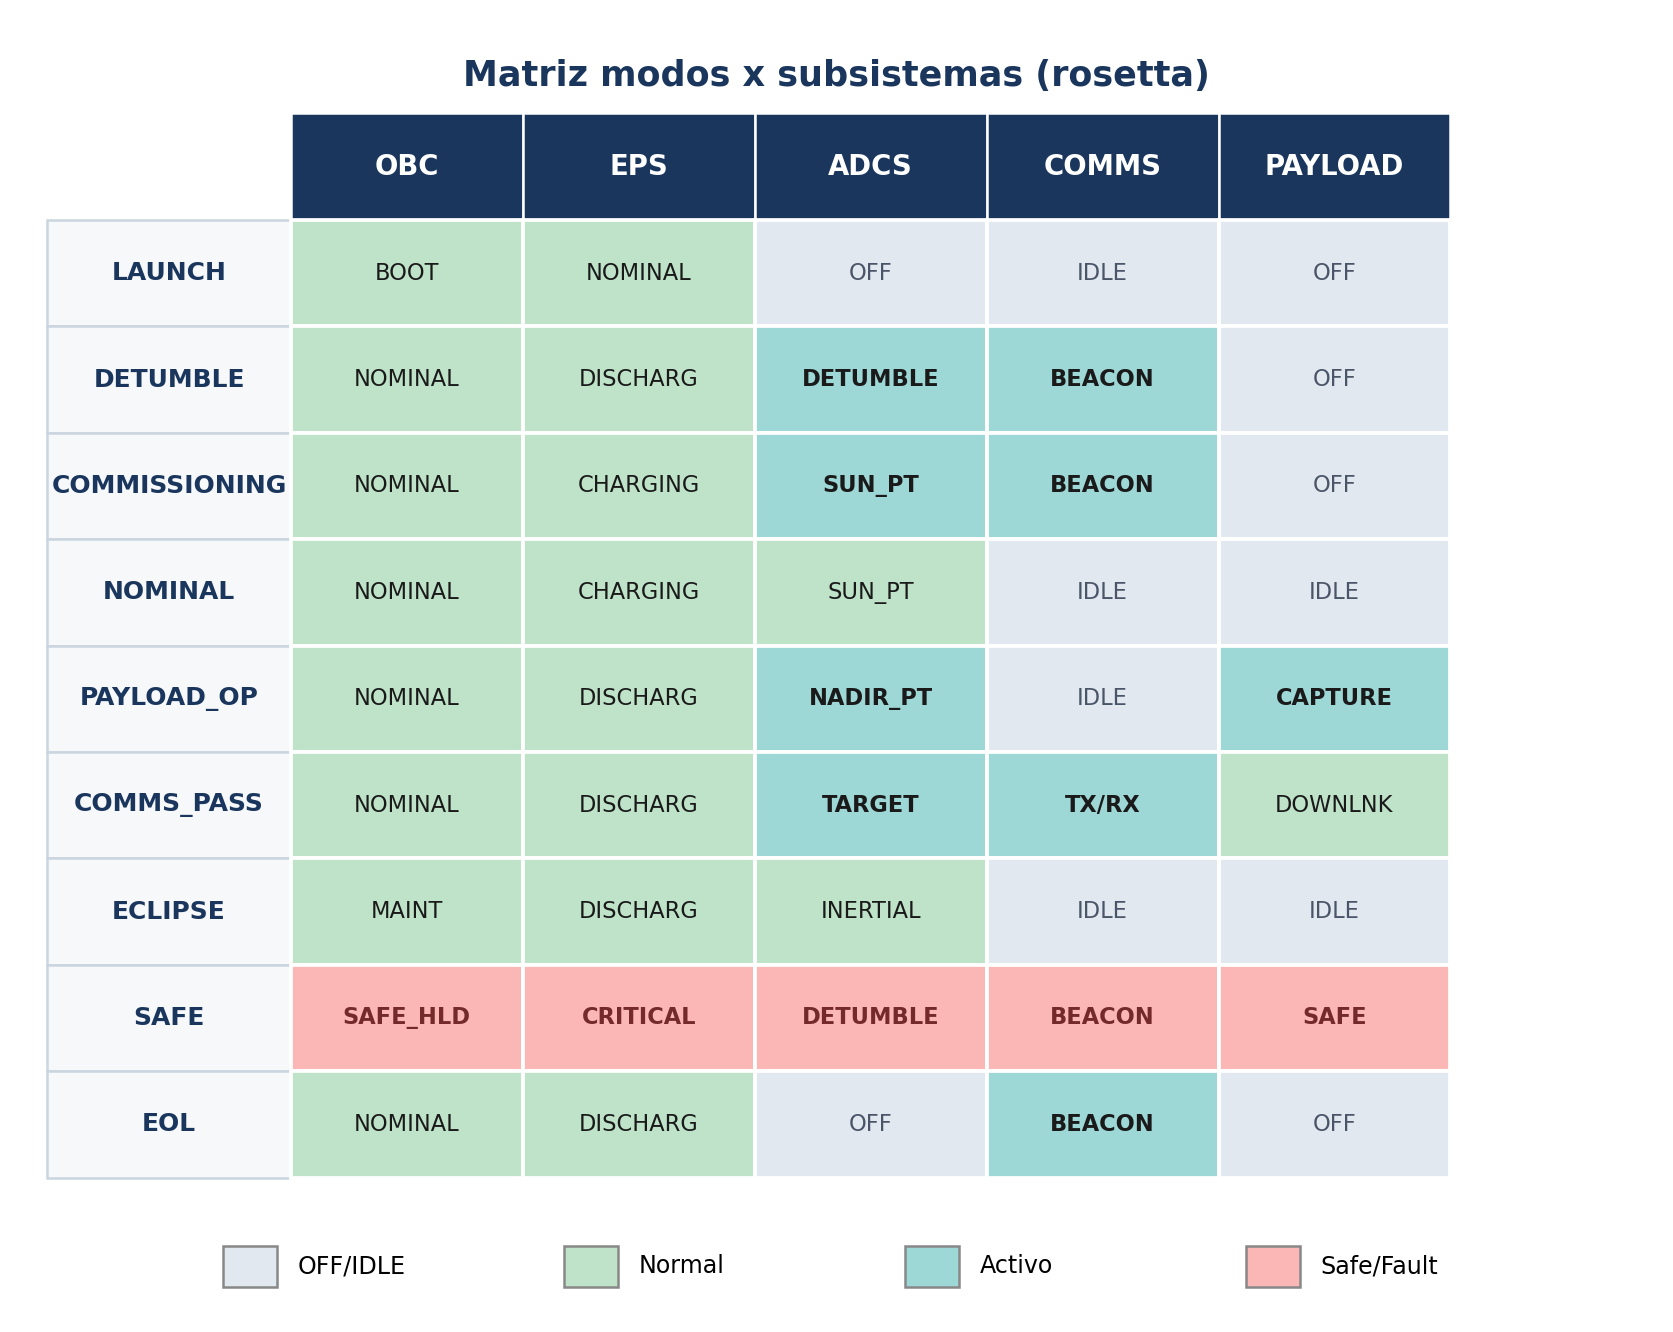
\includegraphics[width=\linewidth]{fig08_matriz.png}
\caption{Matriz que traduce cada modo de mision al estado interno de cada
subsistema. Es el contrato entre los equipos.}
\end{figure}

\section{Como leerla}

Buscas una fila (el modo de mision) y una columna (el subsistema).
La celda te dice en que estado interno tiene que estar ese
subsistema cuando la mision esta en ese modo.

\textbf{Ejemplo:} cuando la mision esta en PAYLOAD\_OP, el ADCS
tiene que estar en NADIR\_POINTING (no en SUN\_POINTING), el EPS
en DISCHARGING (consumimos mas de lo que generamos durante el scan),
y el PAYLOAD en CAPTURE.

\section{Por que esta matriz es importante}

Es el documento que \textbf{evita las discusiones entre equipos}. Si
el lider de ADCS y el lider de Payload no se ponen de acuerdo sobre
si NADIR\_POINTING o TARGET\_POINTING corresponde a PAYLOAD\_OP, la
matriz lo decide. Una vez firmada, es el contrato.

\section{Las reglas de coherencia}

Hay reglas que la matriz debe cumplir para ser consistente:

\begin{enumerate}[leftmargin=2em]
  \item En SAFE, todos los subsistemas deben estar en su estado
    \emph{mas conservador}.
  \item En cualquier modo, EPS debe poder sostener el consumo. Si la
    suma de consumos de cada subsistema en ese modo $>$ la potencia
    generada $+$ la bateria disponible, ese modo es invalido.
  \item Los modos de los subsistemas deben ser alcanzables desde su
    estado anterior (no podemos saltar de IDLE a CAPTURING sin pasar
    por BOOT en el caso del payload, por ejemplo).
\end{enumerate}

\begin{intui}
La matriz se llena \emph{a mano}, en reunion con todos los lideres
tecnicos. Hay 9 modos x 5 subsistemas = 45 celdas. Cada celda lleva
una conversacion: ``en COMMS\_PASS, donde tiene que estar el
payload?'' --- ``en IDLE'' --- ``y si tenemos data pendiente?'' ---
``ah, entonces puede estar en DOWNLINK''. Esa conversacion la haces
una vez, la escribis, y nunca mas vuelve.
\end{intui}

% ============================================================================
\chapter{OBC --- el cerebro central}
% ============================================================================

\begin{figure}[h]
\centering
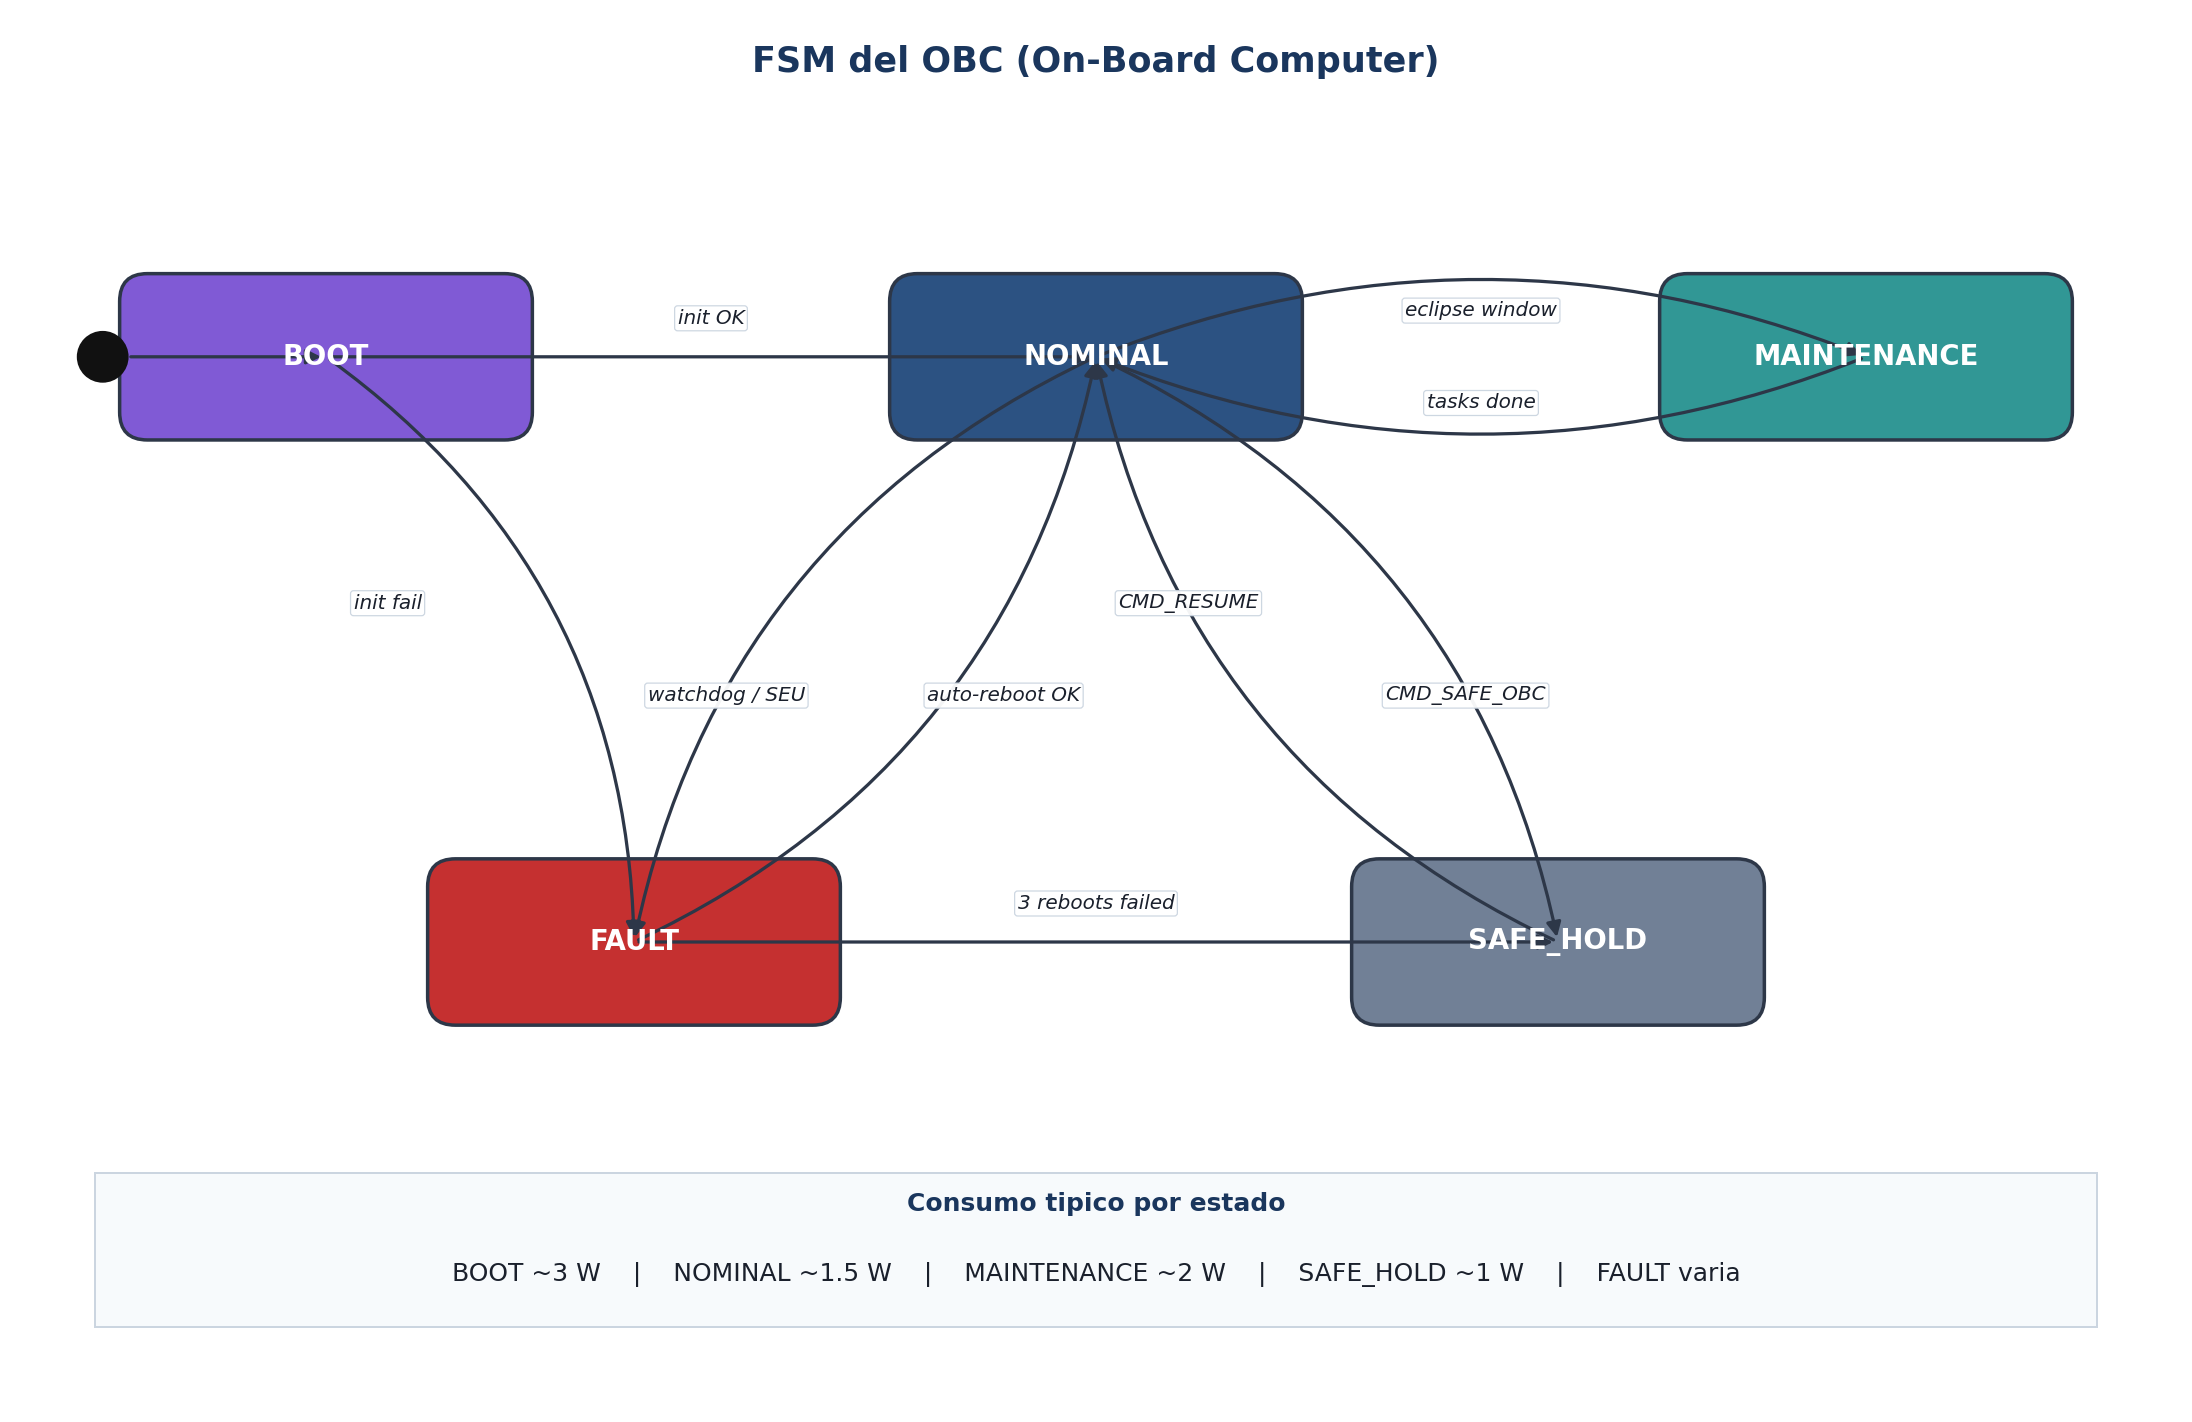
\includegraphics[width=\linewidth]{fig03_obc.png}
\caption{FSM del On-Board Computer. 5 estados, con consumo tipico por estado
en la banda inferior.}
\end{figure}

\section{Que hace el OBC}

El OBC (On-Board Computer) es el \emph{coordinador} del satelite.
Es la pieza que:

\begin{itemize}[leftmargin=2em]
  \item Mantiene el reloj de mision (epoch + uptime).
  \item Decide en que modo de mision esta el satelite.
  \item Recibe comandos del COMMS y los enruta al subsistema correcto.
  \item Recoge telemetria de todos los subsistemas (via I2C, SPI, CAN
    --- depende del diseño) y la prepara para downlink.
  \item Aplica reglas FDIR (\emph{Fault Detection, Isolation and
    Recovery}).
\end{itemize}

En el INTISAT, el OBC NO es el mismo que el CM5 del payload. El OBC
sera un microcontrolador robusto (LPC1768, STM32F4 rad-tolerant, o
similar) que conversa con el CM5 por I2C.

\section{Los 5 estados, en detalle}

\subsection*{BOOT}

\textbf{Que pasa:} kernel arranca, servicios systemd levantan,
chequeo de memoria, chequeo de bus I2C, lectura de configuracion
de NVRAM. Dura $\sim$15 segundos. Consumo: $\sim$3 W (transitorio).

\textbf{Salidas:} \texttt{NOMINAL} si todo OK; \texttt{FAULT} si
init fallido (memoria corrupta, peripheral no responde, etc.).

\subsection*{NOMINAL}

\textbf{Que pasa:} el OBC corre su loop principal: lee telemetria,
verifica reglas FDIR, atiende comandos de COMMS, escribe logs en
ring buffer. Consumo: $\sim$1.5 W.

\textbf{Salidas:} \texttt{MAINTENANCE} (entrada programada en
eclipse), \texttt{FAULT} (watchdog timeout o SEU detectado),
\texttt{SAFE\_HOLD} (comando ground).

\begin{tecnico}
SEU (Single Event Upset) es un bit-flip causado por particulas
cosmicas. En LEO ocurre uno cada $\sim$dia por GB de memoria.
Detectarlo requiere ECC en RAM o checksums en flash. Si el OBC no
tiene ECC, hay que correr \texttt{memtest} periodico (que es lento)
o disenar para que el watchdog reset sea ``barato'' (boot $<$ 30 s).
\end{tecnico}

\subsection*{MAINTENANCE}

\textbf{Que pasa:} tareas de housekeeping. Limpieza de logs viejos,
defrag de la SD/eMMC, escritura de checkpoints, actualizacion de TLEs
si vino comando de ground. Consumo: $\sim$2 W.

Tipicamente se programa para el eclipse, donde no hay otra actividad
util (no se puede hacer payload por que el ADCS no apunta nada).

\textbf{Salida:} \texttt{NOMINAL} cuando termine la lista de tareas.

\subsection*{SAFE\_HOLD}

\textbf{Que pasa:} OBC en consumo minimo, solo acepta una lista
chiquita de comandos:

\begin{itemize}[leftmargin=2em]
  \item \texttt{CMD\_TLM\_DUMP} (volcar telemetria).
  \item \texttt{CMD\_RESUME} (volver a NOMINAL).
  \item \texttt{CMD\_REBOOT} (reset forzado).
\end{itemize}

Consumo: $\sim$1 W. Es el estado del OBC cuando la mision esta en
SAFE.

\textbf{Salida:} \texttt{NOMINAL} con \texttt{CMD\_RESUME}.

\subsection*{FAULT}

\textbf{Que pasa:} el watchdog se disparo o hay un fault. El OBC
intenta auto-reset. Si en 3 intentos no vuelve a NOMINAL, escala a
SAFE\_HOLD para evitar boot-loop infinito.

\textbf{Salidas:} \texttt{NOMINAL} (auto-reset exitoso),
\texttt{SAFE\_HOLD} (3 resets fallidos).

\section{La regla del watchdog}

El watchdog timer es un hardware dedicado (no se puede deshabilitar
desde software facilmente). Cuenta hacia abajo. Si no se ``patea''
(re-arma) en X segundos, resetea el procesador. Esto protege contra
hang del software.

En el INTISAT, el watchdog tipico es de 30--60 s. El loop principal
del OBC debe patearlo cada $\sim$5 s. Si tarda mas de 30 s, asumimos
que el OBC esta colgado y reseteamos.

\begin{cuidado}
NUNCA deshabilites el watchdog ``temporalmente para debug''. Es la
causa numero dos de perdida de mision (numero uno: salir de SAFE
prematuramente). Si necesitas debug local en banco, usa una
configuracion separada con watchdog mas largo.
\end{cuidado}

% ============================================================================
\chapter{EPS --- el corazon energetico}
% ============================================================================

\begin{figure}[h]
\centering
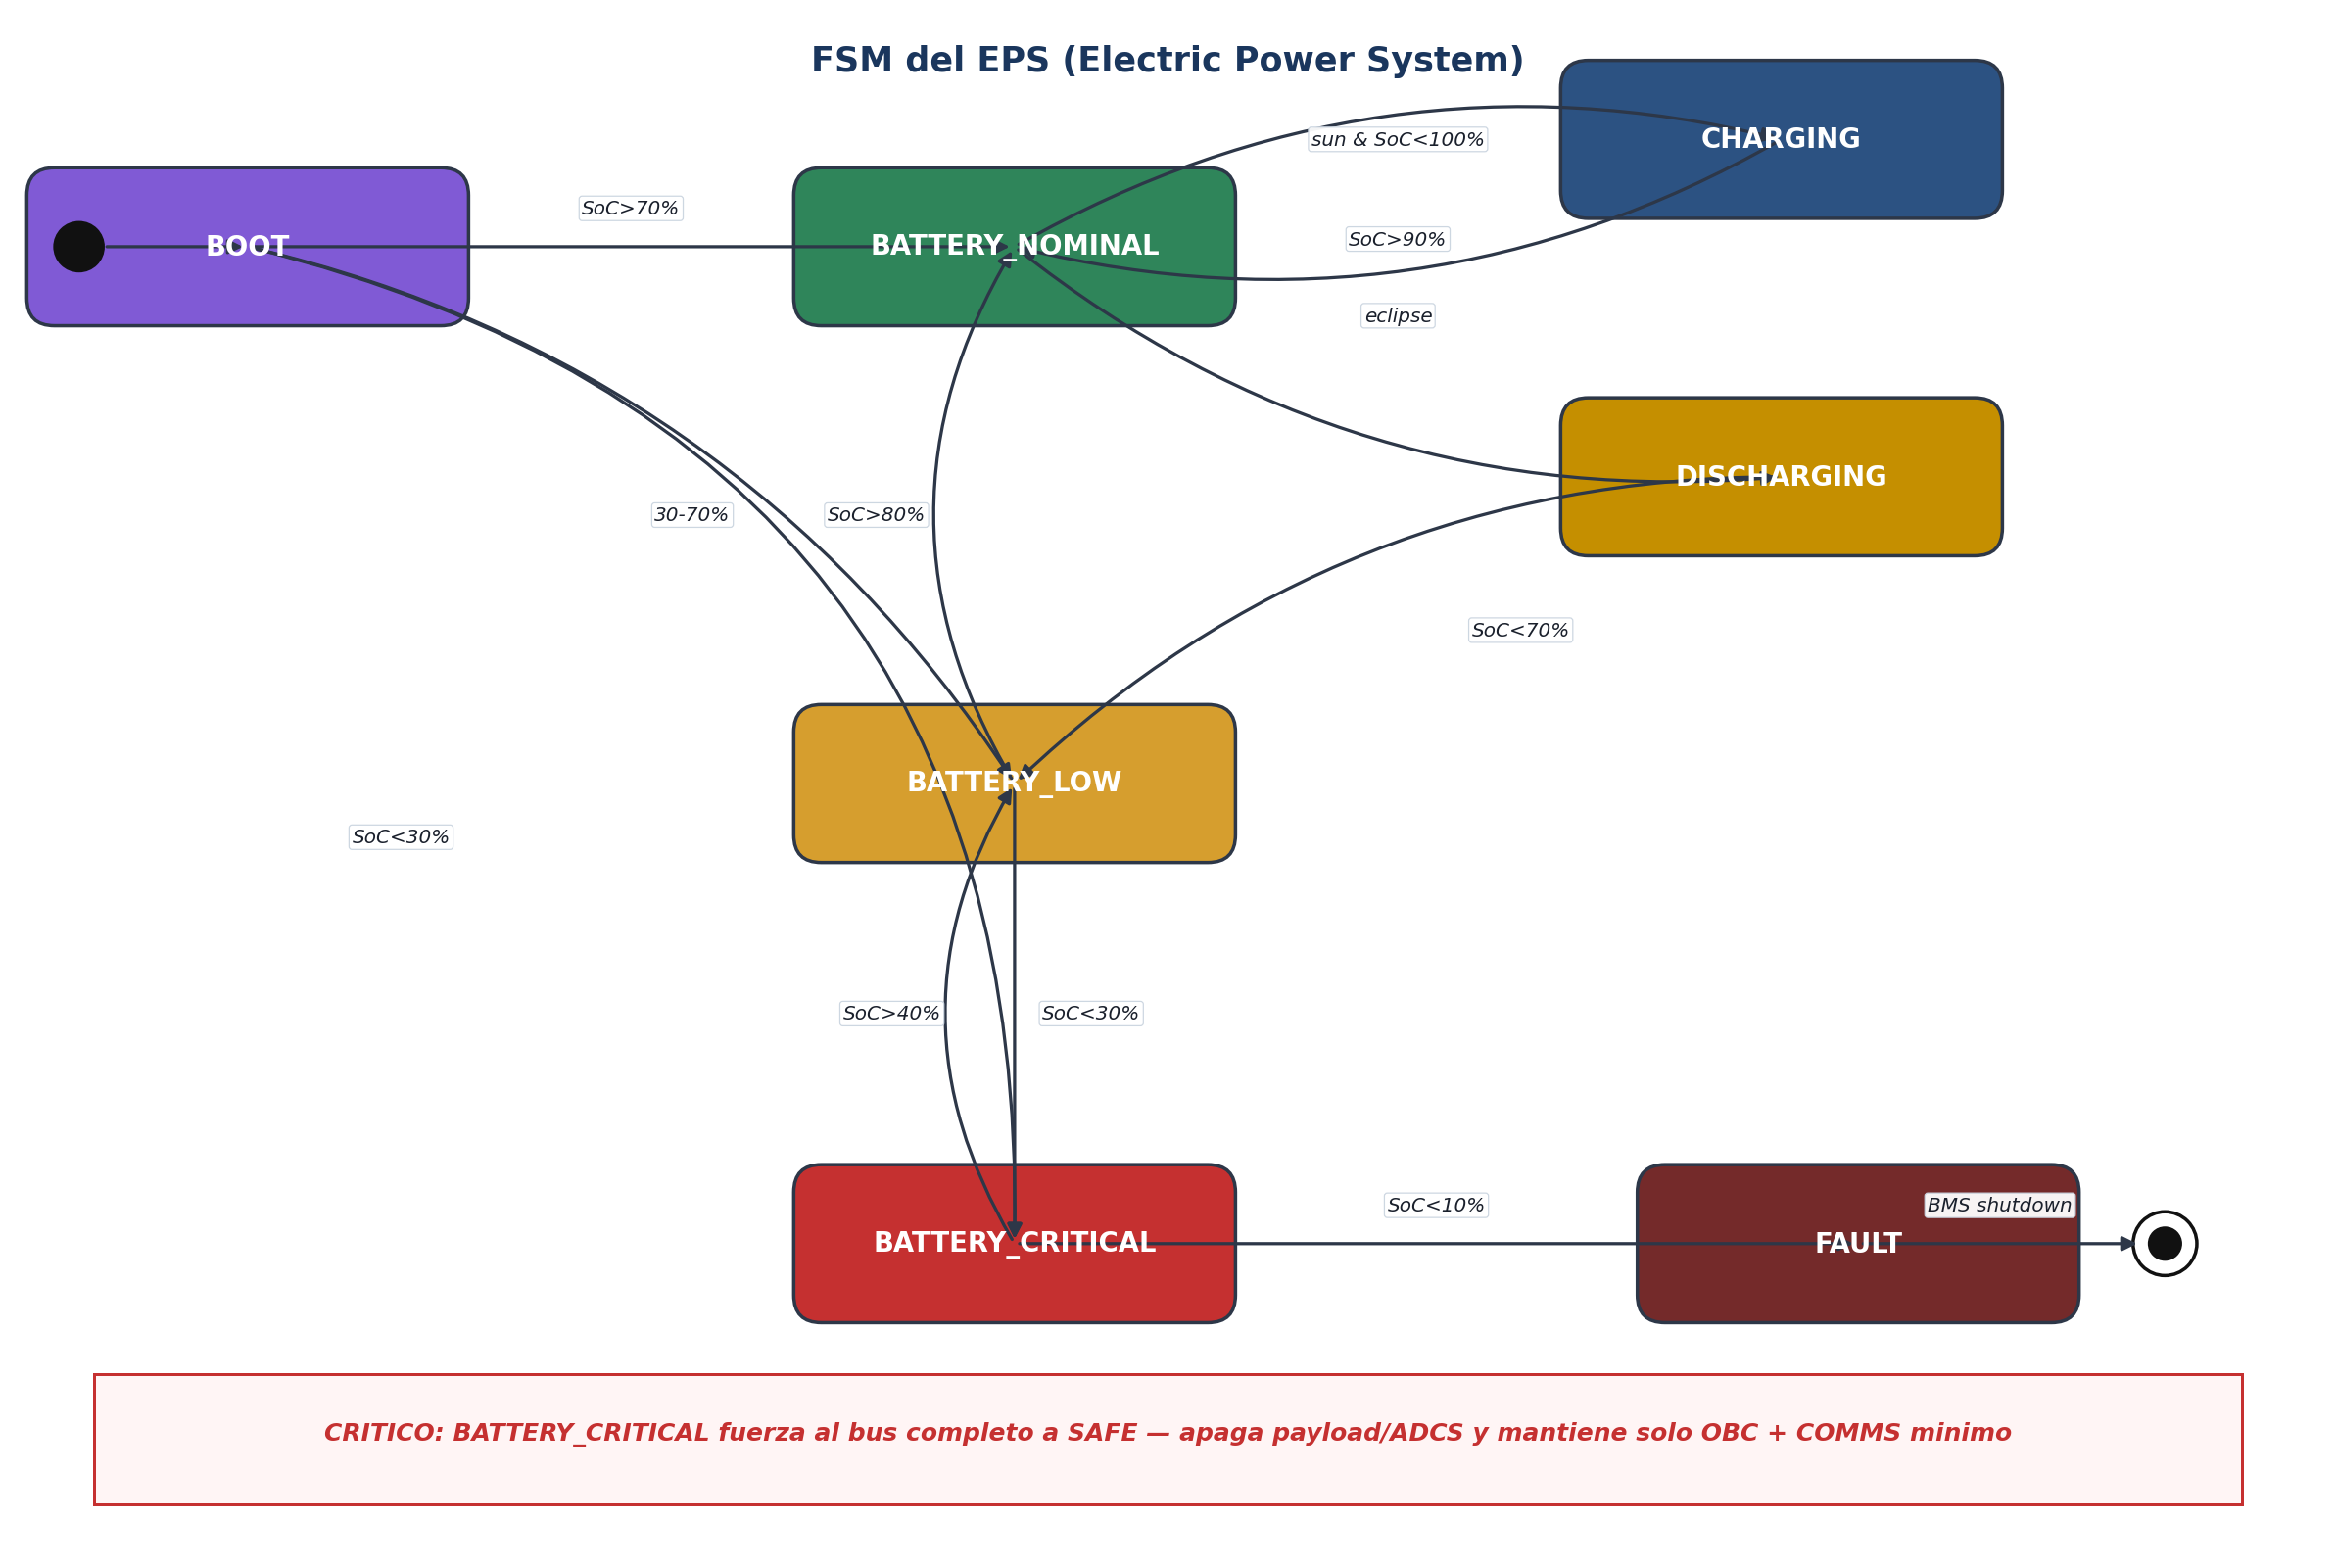
\includegraphics[width=\linewidth]{fig04_eps.png}
\caption{FSM del EPS. Los estados de bateria forman una cadena que va de
NOMINAL hasta CRITICAL, con la posibilidad de FAULT irrecuperable si
SoC cae por debajo de 10\%.}
\end{figure}

\section{Por que EPS es el subsistema mas critico}

Porque si EPS falla, todo lo demas se apaga, ni siquiera tenes
telemetria para diagnosticar el fallo. EPS tiene autoridad para:

\begin{itemize}[leftmargin=2em]
  \item Forzar al OBC a SAFE\_HOLD si SoC $< $ umbral.
  \item Apagar rails de potencia no esenciales.
  \item Reactivar rails despues de un fault transitorio.
  \item Reportar telemetria de salud propia incluso si OBC esta caido.
\end{itemize}

En arquitecturas profesionales (e.g., GomSpace NanoPower P31u), el
EPS tiene su propio microcontrolador (TI MSP430 tipico) totalmente
independiente del OBC.

\section{Los 7 estados, en detalle}

\subsection*{BOOT}

Al power-on, el EPS lee SoC de la bateria (via gauge dedicado, e.g.,
LTC2942) y decide en cual de los 3 estados de bateria arrancar:

\begin{itemize}[leftmargin=2em]
  \item SoC $>$ 70\% $\to$ \texttt{BATTERY\_NOMINAL}.
  \item 30\% $<$ SoC $<$ 70\% $\to$ \texttt{BATTERY\_LOW} (no enciende
    payload).
  \item SoC $<$ 30\% $\to$ \texttt{BATTERY\_CRITICAL} (solo OBC + COMMS).
\end{itemize}

\subsection*{BATTERY\_NOMINAL}

Estado feliz. Todos los rails alimentados. Es el ``IDLE'' del EPS.
Subestados: CHARGING (si vemos sol y SoC $<$ 100\%) o DISCHARGING (si
estamos en eclipse).

\subsection*{CHARGING / DISCHARGING}

No son ``modos distintos'' del EPS desde el punto de vista del
satelite; son flags internos. El EPS sigue siendo BATTERY\_NOMINAL
externamente. Internamente es importante para el MPPT y para
predecir cuanta autonomia queda.

\subsection*{BATTERY\_LOW}

Cuando SoC cae por debajo de 70\% en DISCHARGING (eclipse largo o
consumo alto). El EPS \textbf{notifica al OBC} para que considere
suspender operaciones no esenciales (e.g., no arrancar un payload
scan nuevo).

Para volver a NOMINAL hace falta SoC $>$ 80\% (hysteresis para evitar
chattering entre estados).

\subsection*{BATTERY\_CRITICAL}

SoC $<$ 30\%. Esto es serio. El EPS:

\begin{enumerate}[leftmargin=2em]
  \item Manda evento de SAFE al OBC (que pasa todo el satelite a SAFE).
  \item Apaga rails de payload, ADCS no esencial, etc.
  \item Mantiene solo OBC en SAFE\_HOLD + COMMS en BEACON.
\end{enumerate}

Para salir de CRITICAL hace falta SoC $>$ 40\% (recuperacion lenta
con luz solar).

\subsection*{FAULT}

SoC $<$ 10\%. El BMS (Battery Management System) corta el bus
principal para proteger las celdas de over-discharge. Esto es
\textbf{normalmente irrecuperable} --- el satelite queda sin
telemetria. Es un evento ``mission end''.

\begin{cuidado}
Las celdas Li-ion sufren daño permanente si bajan de 2.5 V/celda.
El BMS corta a $\sim$2.7 V/celda como margen. Una vez que cae mas
bajo, aunque vuelva la luz solar, la celda puede no aceptar carga
o aceptar mucho menos de la capacidad original. Por eso CRITICAL
$\to$ FAULT es a 10\% (no a 5\%): para tener margen de la latencia
de respuesta del BMS.
\end{cuidado}

\section{La estimacion del SoC}

El SoC (State of Charge) NO se mide directamente. Se estima. Hay
tres metodos comunes:

\begin{enumerate}[leftmargin=2em]
  \item \textbf{Coulomb counting:} integrar la corriente entrante y
    saliente. Precisa pero acumula error (drift) sin
    recalibracion.
  \item \textbf{Open-Circuit Voltage (OCV):} medir voltaje sin carga.
    Preciso pero requiere periodos de no-current (eclipse).
  \item \textbf{Modelo Kalman:} combina coulomb counting con OCV.
    Es lo que usan los gauges modernos (LTC2942, MAX17048).
\end{enumerate}

% ============================================================================
\chapter{ADCS --- a donde apunta el satelite}
% ============================================================================

\begin{figure}[h]
\centering
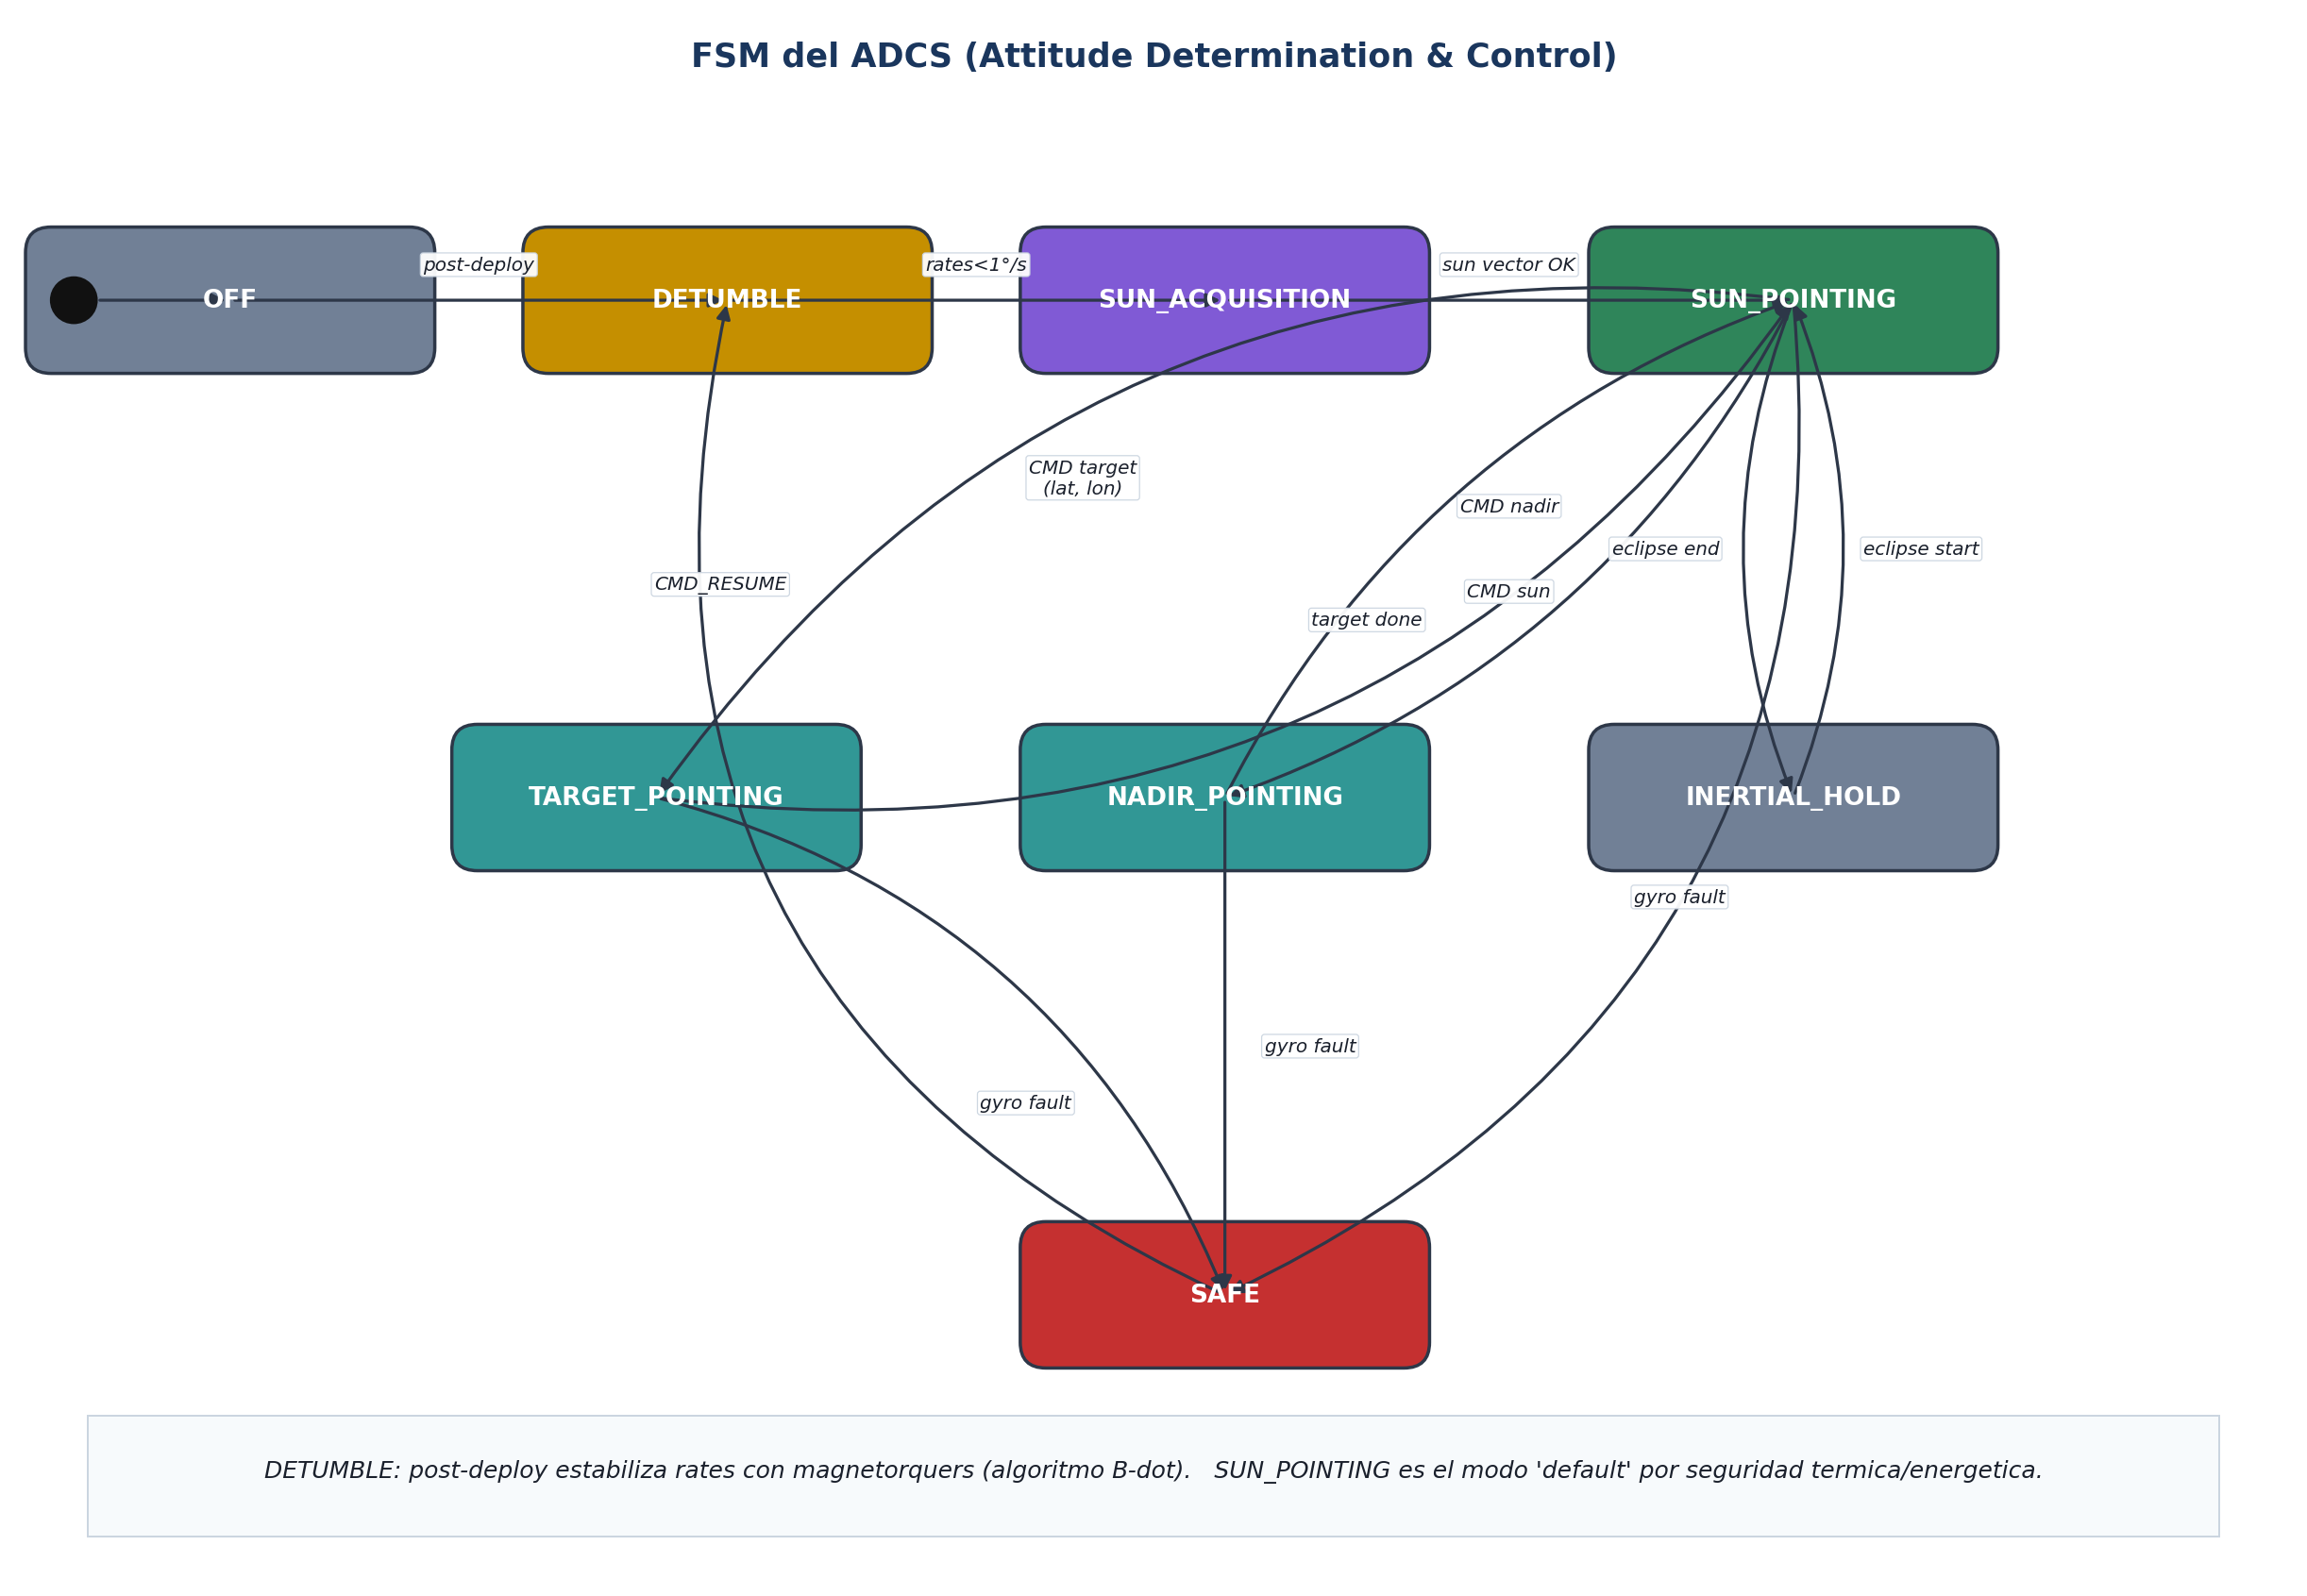
\includegraphics[width=\linewidth]{fig05_adcs.png}
\caption{FSM del ADCS. SUN\_POINTING es el modo ``default'' (por seguridad
termica). Cualquier modo activo (NADIR/TARGET) puede volver via SUN\_POINTING.}
\end{figure}

\section{Por que SUN\_POINTING es el default}

Toda FSM tiene un ``estado seguro pero util''. Para el ADCS, ese es
SUN\_POINTING. Razones:

\begin{enumerate}[leftmargin=2em]
  \item \textbf{Energia:} si los paneles apuntan al sol, generamos
    corriente. Si apuntamos a otro lado, descargamos bateria.
  \item \textbf{Termica:} apuntar al sol mantiene una cara caliente
    y otra fria, en lugar de barrer todo el satelite por toda la
    expansion termica.
  \item \textbf{Conocido:} el vector solar es facil de calcular con
    Kepler. El vector nadir requiere conocer altitud y attitude. El
    vector target requiere conocer la posicion del ground station
    \emph{y} la del satelite simultaneamente.
\end{enumerate}

\section{Los 8 estados}

\subsection*{OFF}

ADCS apagado. Estado en LAUNCH (antes de despliegue) y en EOL.

\subsection*{DETUMBLE}

Activacion del algoritmo B-dot. Magnetorquers comandados a frenar
el spin residual. Sin reaction wheels en esta fase (los wheels
requieren actitud conocida; aqui no la tenemos).

\subsection*{SUN\_ACQUISITION}

Una vez detumbled, buscar el vector solar. Si los sensores de sol
no detectan flujo, el satelite hace un spin lento ($\sim$2 \textdegree/s)
para barrer el cielo.

\subsection*{SUN\_POINTING}

El modo default. Reaction wheels (o magnetorquers) mantienen los
paneles solares ortogonales al vector solar. Precision tipica:
$\pm$2--5 \textdegree.

\subsection*{NADIR\_POINTING}

Para PAYLOAD\_OP (microscopia mirando hacia Tierra). Apuntar el eje
+Z hacia nadir. Precision requerida depende del payload; para
microscopia FPM lensless el requirement es relativamente laxo
($\pm$1--2 \textdegree).

\subsection*{TARGET\_POINTING}

Para COMMS\_PASS, apuntar la antena hacia el ground station. Esto
requiere TLE actualizado y conocer la posicion del ground station.
Precision tipica $\pm$0.5 \textdegree~ para antena directiva.

\subsection*{INERTIAL\_HOLD}

Durante eclipse, mantener actitud actual sin gastar energia en
correcciones agresivas. Wheels se mantienen en momentum bajo.

\subsection*{SAFE}

Cualquier fault del giroscopo o magnetometro principal. Vuelve a
DETUMBLE para recuperar baseline.

\section{Hardware tipico de un ADCS CubeSat}

\begin{itemize}[leftmargin=2em]
  \item \textbf{Magnetometro:} HMC5883L, MMC5983MA. 3 ejes.
  \item \textbf{Giroscopo:} L3G4200D, BMI088. 3 ejes.
  \item \textbf{Sensor de sol:} fotodiodos en cada cara (6 caras) o
    \emph{sun sensors} (NanoSSOC-D60, etc.).
  \item \textbf{Magnetorquers:} bobinas en X, Y, Z. Tipicamente 0.1--0.2 Am$^2$.
  \item \textbf{Reaction wheels:} opcional. Para precision $<$ 1\textdegree.
\end{itemize}

% ============================================================================
\chapter{COMMS --- la voz del satelite}
% ============================================================================

\begin{figure}[h]
\centering
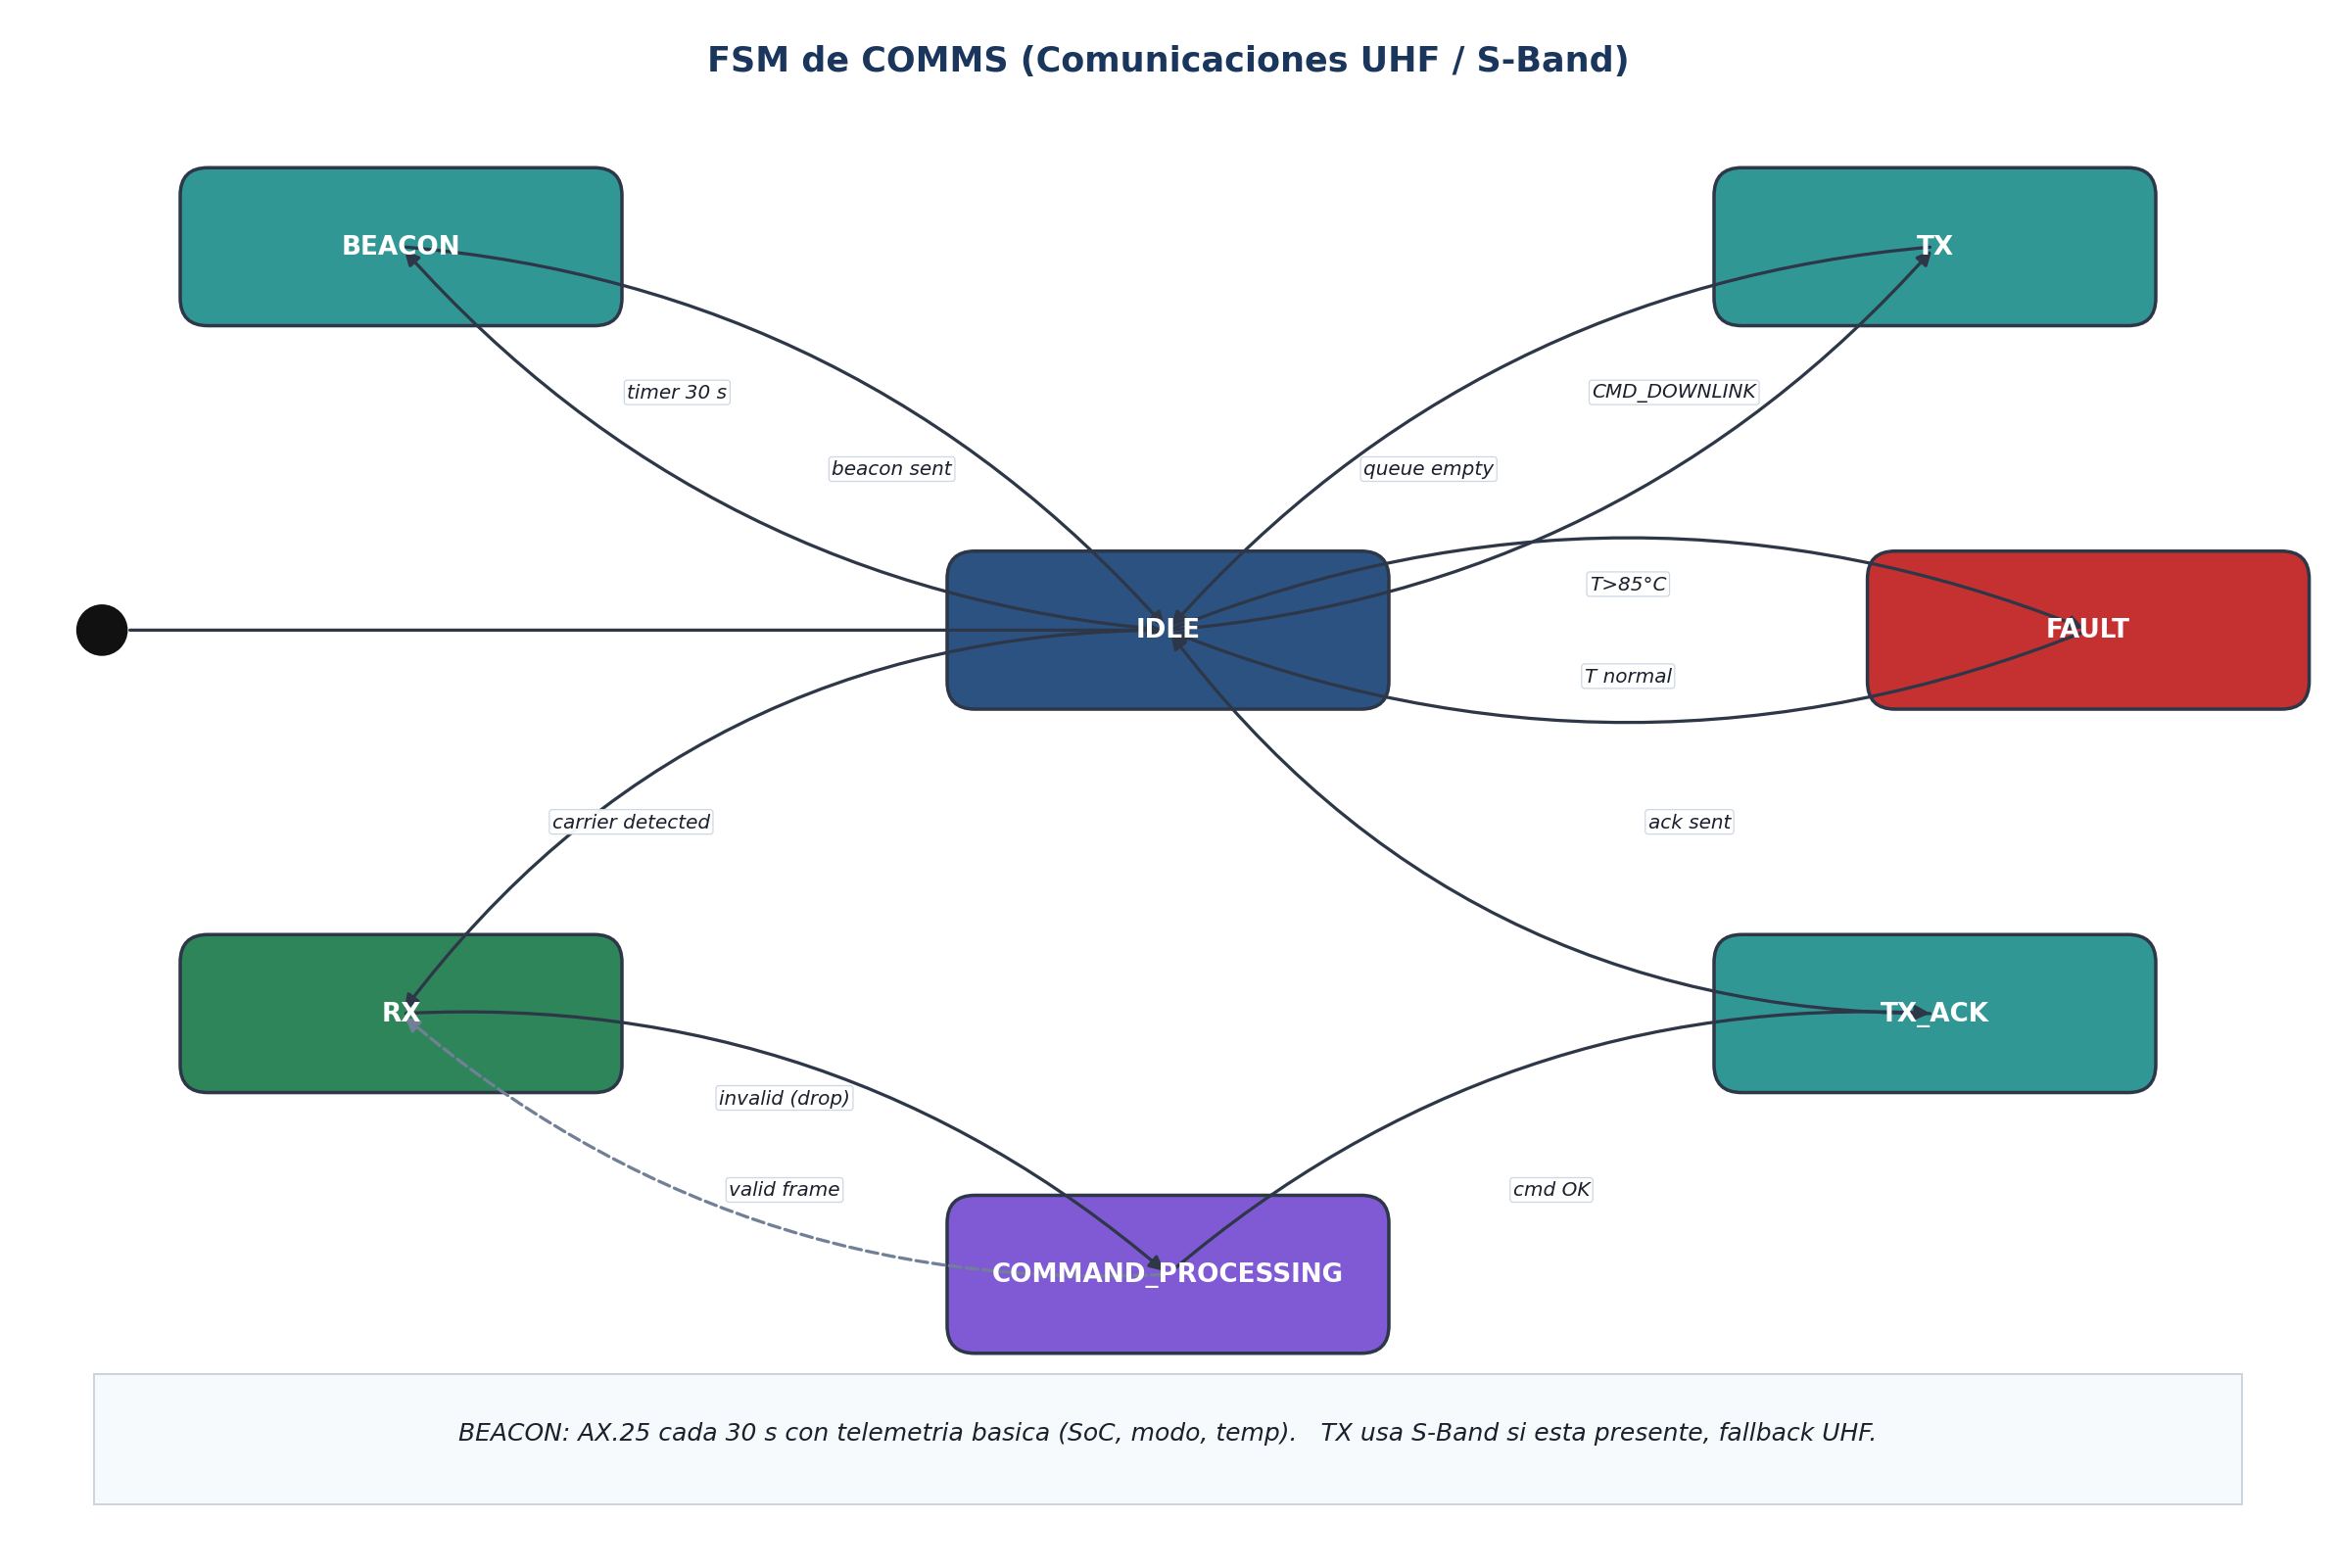
\includegraphics[width=\linewidth]{fig06_comms.png}
\caption{FSM de comunicaciones. IDLE es el hub central; BEACON, RX, TX y
los caminos de comando giran alrededor.}
\end{figure}

\section{Las dos bandas tipicas}

\begin{itemize}[leftmargin=2em]
  \item \textbf{UHF (430--440 MHz):} amateur radio band, sin licencia
    comercial. Throughput 1.2--9.6 kbps. Antena omnidireccional.
    Usado para comandos y beacon.
  \item \textbf{S-Band (2200--2300 MHz):} requiere licencia. Throughput
    hasta 1 Mbps con antena directiva. Usado para downlink de datos
    (imagenes, video).
\end{itemize}

INTISAT comienza con solo UHF. S-Band se agregaria en una version
futura si el volumen de datos lo justifica.

\section{Los 7 estados}

\subsection*{IDLE}

Radio encendido pero sin actividad. Receiver escuchando, transmitter
apagado. Consumo bajo. Es el ``hub'' de la FSM de COMMS.

\subsection*{BEACON}

Cada 30 s, transmite paquete corto AX.25 con telemetria minima: SoC,
modo de mision, temperatura, contador de uptime. Permite que cualquier
radioaficionado en el mundo confirme que el satelite esta vivo.

\subsection*{RX}

Carrier detectado. Receptor demodula y entrega paquetes al
processor para decodificacion.

\subsection*{COMMAND\_PROCESSING}

Frame valido recibido. Verifica CRC, autenticacion (HMAC), y
secuencia anti-replay. Si pasa, ejecuta. Si falla, descarta y vuelve
a RX.

\subsection*{TX\_ACK}

Despues de ejecutar un comando, envia ack con resultado.

\subsection*{TX}

Comando explicito \texttt{CMD\_DOWNLINK} dispara una sesion de
transmision. Vacia la queue de telemetria/datos. Si tiene S-Band,
usa S-Band; fallback UHF.

\subsection*{FAULT}

Temperatura del PA (Power Amplifier) sobre 85 \textdegree C, o
SWR muy alto (antena rota o conector flojo). Se apaga TX hasta
que la temperatura normalice.

\section{Por que BEACON es tan importante}

Un satelite que beaconea es un satelite vivo. Aunque el resto este
caido, mientras el beacon llegue a tierra:

\begin{itemize}[leftmargin=2em]
  \item Sabemos donde esta orbitando (refinamos TLE con doppler).
  \item Sabemos que la bateria no esta muerta.
  \item Tenemos un canal para diagnosticar.
\end{itemize}

Diseñar BEACON como hardware con un timer dedicado (no dependiente
del OBC) es una buena practica defensiva.

% ============================================================================
\chapter{PAYLOAD --- el caso INTISAT}
% ============================================================================

\begin{figure}[h]
\centering
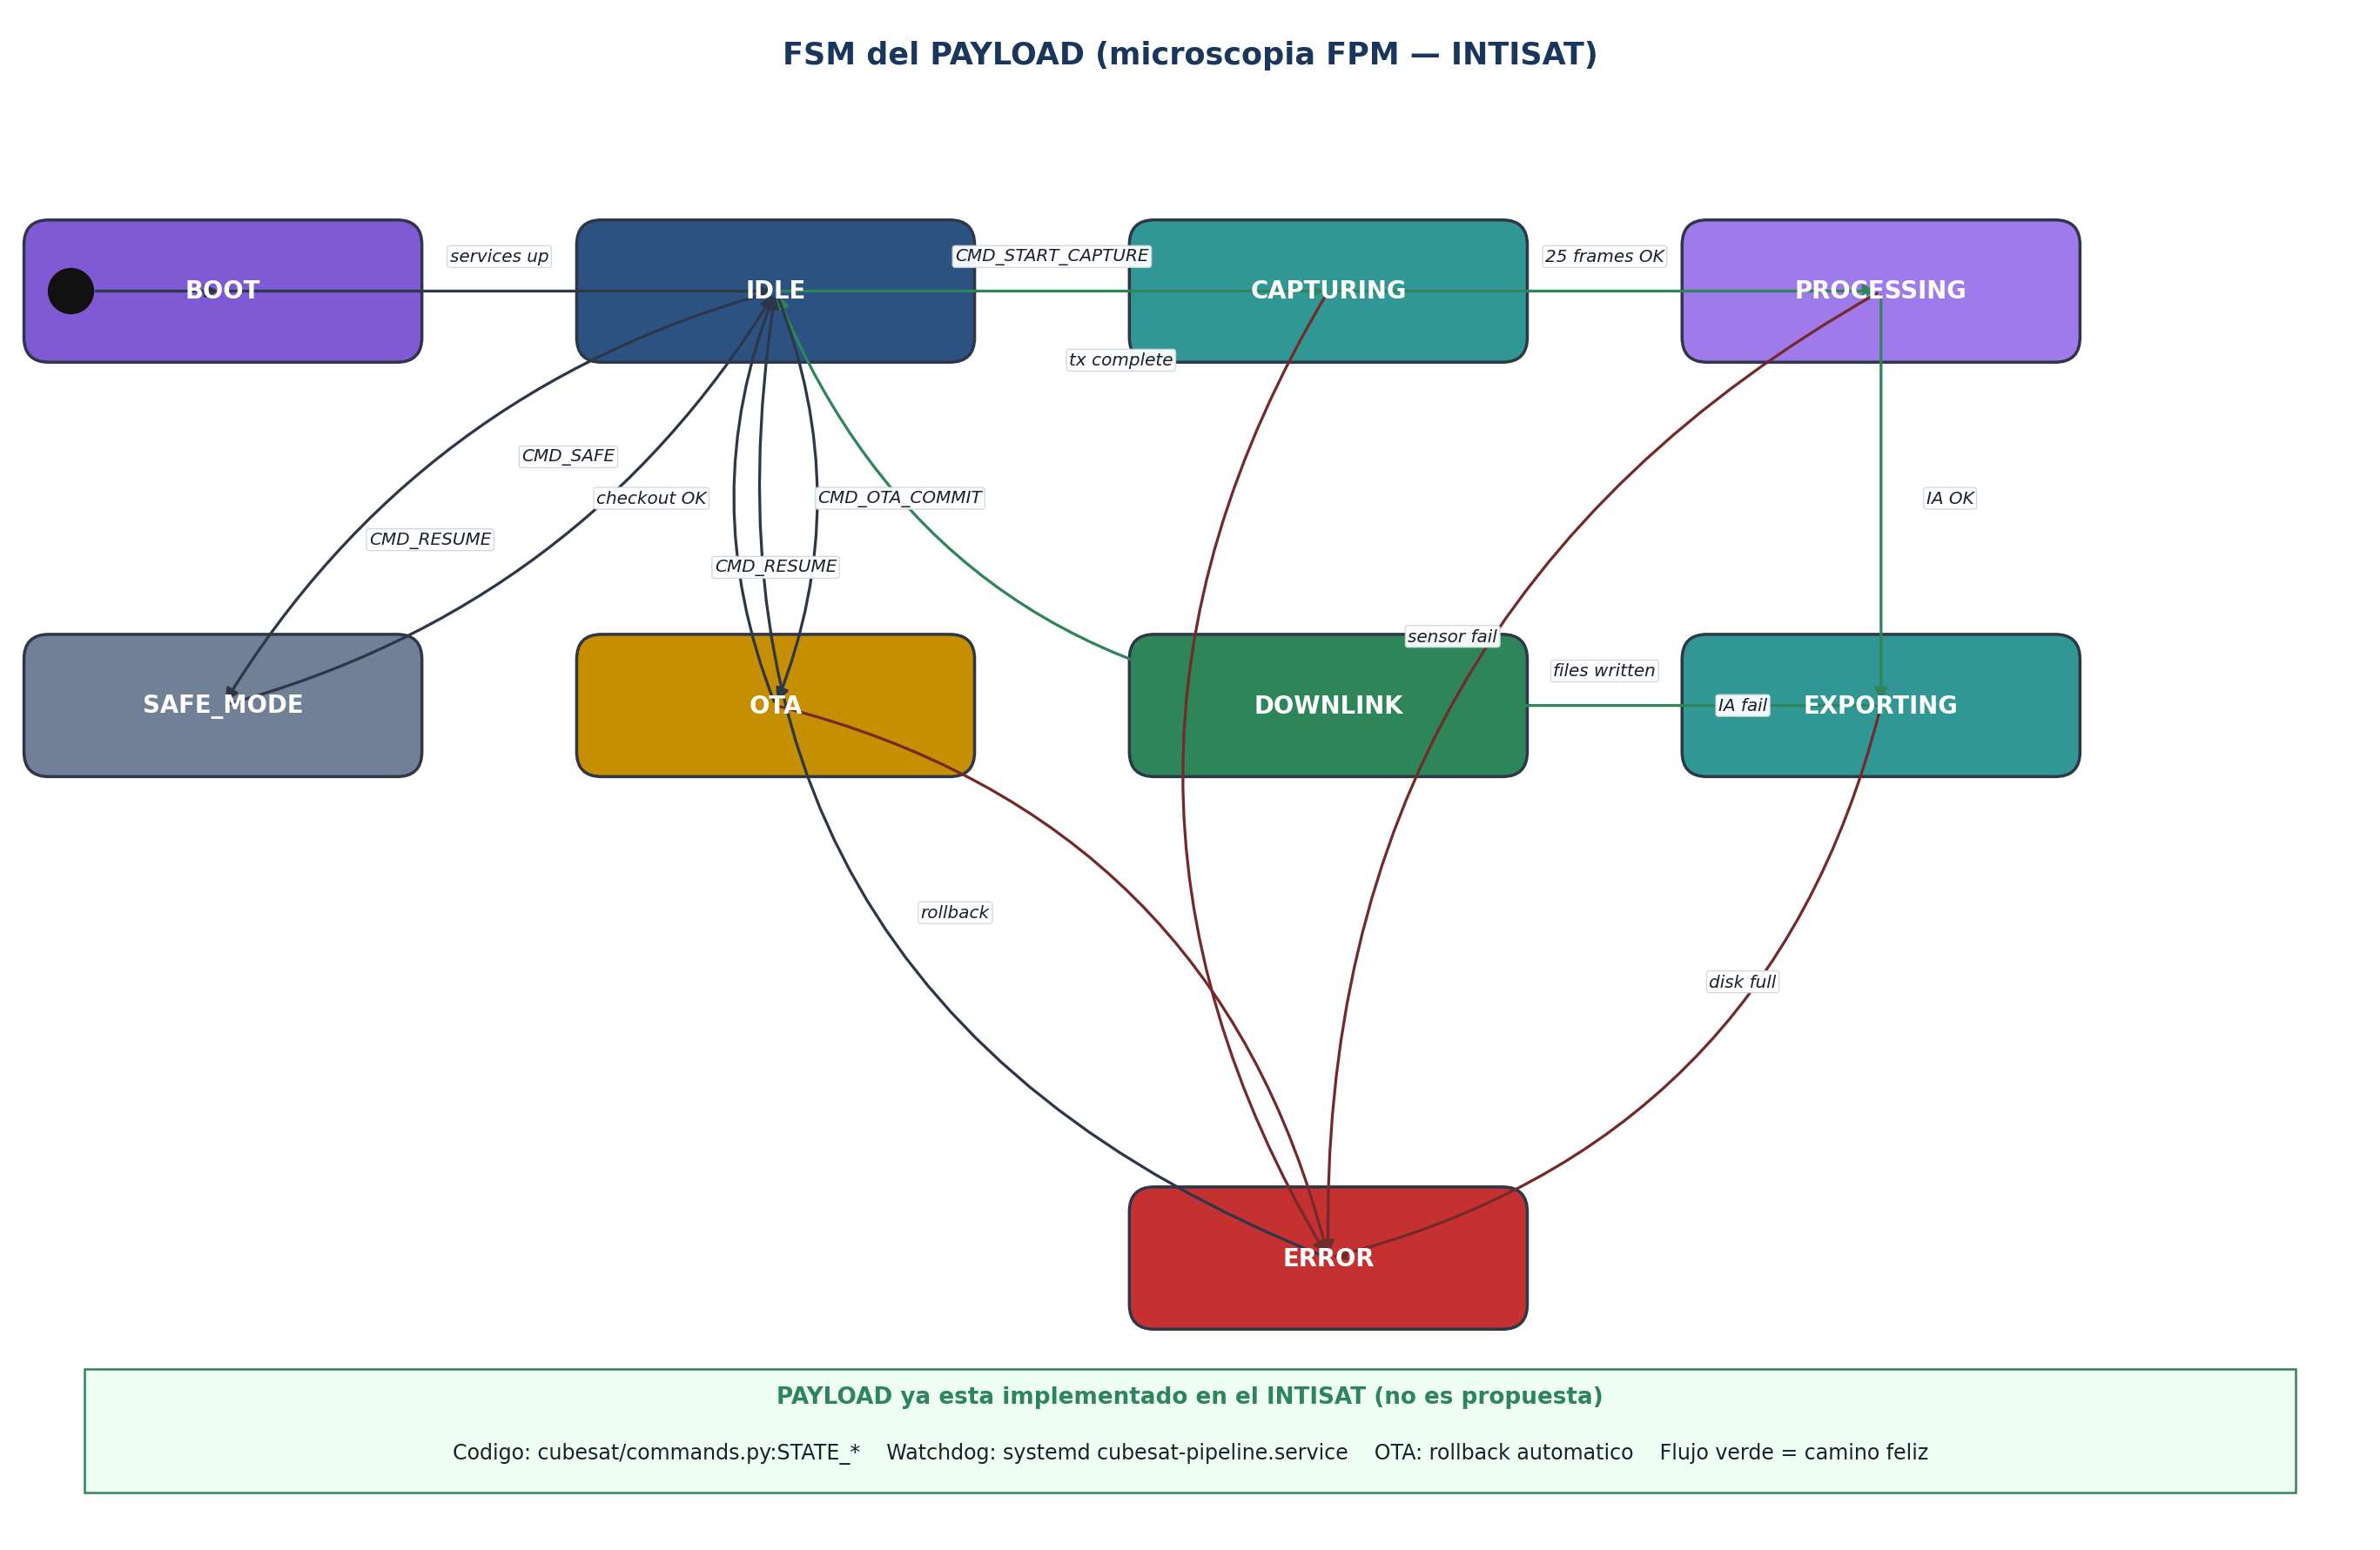
\includegraphics[width=\linewidth]{fig07_payload.png}
\caption{FSM del payload de microscopia FPM del INTISAT. El camino verde es
el ``happy path''. Errores caen a ERROR central, recuperable via CMD\_RESUME.}
\end{figure}

\section{Por que este es el subsistema mas avanzado}

Porque ya esta implementado. No es propuesta. Esta corriendo en el
laboratorio, en una Raspberry Pi 5, con codigo en
\texttt{cubesat/}.

\begin{logrado}
La FSM del payload existe en codigo, no solo en este documento. Los
estados estan en \texttt{cubesat/commands.py:STATE\_*}. Las
transiciones estan en \texttt{cubesat/daemon.py}. El watchdog esta
en \texttt{cubesat-pipeline.service} (systemd).
\end{logrado}

\section{Los 9 estados, en detalle}

\subsection*{BOOT}

Inicializacion al power-on:

\begin{enumerate}[leftmargin=2em]
  \item Levantar servicios systemd (\texttt{cubesat-pipeline.service}).
  \item Cargar configuracion de \texttt{config.yaml}.
  \item Inicializar OV5647 (libcamera \texttt{rpicam-hello} para
    sanity check).
  \item Inicializar OLED SSD1351 (luma.oled).
  \item Inicializar INA219 (i2c-tools, address 0x40).
  \item Conectar a I2C slave con OBC (pigpio bsc, address 0x42).
\end{enumerate}

Tipicamente $\sim$30 segundos. Consumo: $\sim$5 W transitorio.

\textbf{Salidas:} \texttt{IDLE} si todo OK; \texttt{ERROR} si algun
init fallido.

\subsection*{IDLE}

Pipeline corriendo pero sin captura. OLED muestra estado. INA219
sampling cada 5 s. Esperando comandos.

Consumo $\sim$2 W.

\subsection*{CAPTURING}

\texttt{CMD\_START\_CAPTURE} recibido. Secuencia:

\begin{enumerate}[leftmargin=2em]
  \item Recibir parametros (ISO, exposure, num\_frames).
  \item Activar OLED para iluminacion del DUT (Device Under Test).
  \item Cambiar mascara (si aplica, mecanismo MEMS o por filtro
    movil).
  \item Capturar N frames con OV5647.
  \item Guardar raws en \texttt{/scans/raw/\{timestamp\}/}.
\end{enumerate}

Consumo $\sim$6 W (sensor + OLED + procesamiento ligero).

\textbf{Salidas:} \texttt{PROCESSING} al completar N frames;
\texttt{ERROR} si sensor falla.

\subsection*{PROCESSING}

Inferencia con la red. Tres pasos:

\begin{enumerate}[leftmargin=2em]
  \item Stack: alinear los N frames (registracion).
  \item Reconstruccion FPM o super-resolucion (Real-ESRGAN-x4).
  \item Guardar resultado en \texttt{/scans/processed/\{ts\}/}.
\end{enumerate}

Consumo $\sim$8 W pico (CPU saturada, sin GPU acelerada en RPi 5
por ahora). Tiempo: $\sim$60--90 s por scan de 25 frames.

\textbf{Salidas:} \texttt{EXPORTING} si IA OK; \texttt{ERROR} si
inferencia falla (e.g., out-of-memory).

\subsection*{EXPORTING}

Empaquetado para downlink:

\begin{enumerate}[leftmargin=2em]
  \item Comprimir imagen final (PNG o JPEG).
  \item Generar metadatos (timestamp, ISO, exposure, frame count,
    quality metric).
  \item Escribir tar.gz en \texttt{/downlink/queue/}.
\end{enumerate}

Consumo $\sim$2 W. Tiempo: $\sim$10 s.

\subsection*{DOWNLINK}

Negociacion con OBC para transmitir. El OBC pregunta al payload
``tenes datos?'' periodicamente; cuando el payload reporta
\texttt{queue\_size $>$ 0}, el OBC programa el proximo COMMS\_PASS.

\subsection*{SAFE\_MODE}

Comando \texttt{CMD\_SAFE} desde OBC. Payload baja al consumo
minimo: $\sim$1 W. OV5647 OFF, OLED OFF, solo daemon corriendo
para escuchar \texttt{CMD\_RESUME}.

\subsection*{OTA}

Comando \texttt{CMD\_OTA\_COMMIT}. El payload aplica un update de
software preinstalado (en un slot B, A/B booting). Si el boot del
nuevo slot falla, vuelve automaticamente al slot anterior (rollback).

\subsection*{ERROR}

Cualquier fault. Mantiene el modo hasta que llegue \texttt{CMD\_RESUME}
desde tierra. Importante: ERROR NO es lo mismo que SAFE\_MODE ---
ERROR mantiene logs detallados del fault para diagnostico; SAFE\_MODE
es solo bajar consumo.

\begin{payloadbox}
La diferencia entre ERROR y SAFE\_MODE es clave: ERROR implica
``algo se rompio, no toques'', SAFE\_MODE implica ``estoy en pausa
voluntaria''. Operacionalmente: si ves ERROR en telemetria, tenes
que diagnosticar (descargar logs, hacer un dump). Si ves SAFE\_MODE,
solo mandas CMD\_RESUME cuando quieras.
\end{payloadbox}

\section{El camino feliz vs los caminos de error}

En el diagrama de la figura, las flechas \emph{verdes} forman el
``happy path'' que va de IDLE a IDLE via todos los pasos del scan.
Las flechas \emph{rojas} son los desvios a ERROR. La unica salida de
ERROR es \texttt{CMD\_RESUME} desde tierra.

% ============================================================================
\chapter{Comparacion contra el INTISAT actual}
% ============================================================================

\section{Estado del arte por subsistema}

\begin{longtable}{p{2.5cm}p{3cm}p{6cm}}
\toprule
\textbf{Subsistema} & \textbf{Madurez} & \textbf{Estado actual} \\
\midrule \endhead
PAYLOAD & FSM completa (80\%) &
  Codigo en \texttt{cubesat/commands.py}, daemon corriendo,
  watchdog systemd, OTA rollback. Falta validacion vibracion +
  thermal. \\
\midrule
OBC & Propuesta (20\%) &
  Solo este documento. Hardware aun no definido (LPC vs STM32).
  Sin codigo. \\
\midrule
EPS & Propuesta (20\%) &
  Especificacion teorica. Se evalua GomSpace P31u vs custom.
  Sin codigo. \\
\midrule
ADCS & Propuesta (20\%) &
  Especificacion teorica. Sensores comprados (magnetometro,
  giroscopo); falta integrar. \\
\midrule
COMMS & Propuesta (20\%) &
  Especificacion teorica. Radio UHF comprado, antena en diseno
  mecanico. \\
\midrule
MISION & Propuesta (20\%) &
  Documento describe los 8 modos, falta validar con stakeholders
  y simular. \\
\bottomrule
\end{longtable}

\section{Plan sugerido}

\subsection*{Sprint 1 (proximas 2 semanas)}

\begin{enumerate}[leftmargin=2em]
  \item \textbf{Reunion de matriz} (4 hs). Todos los lideres tecnicos
    + lider de proyecto. Validar las 45 celdas de la matriz capitulo 4.
  \item Firmar la matriz como version 1.0.
  \item Cada lider crea un Issue en GitHub para implementar la FSM
    de su subsistema.
\end{enumerate}

\subsection*{Sprint 2 (siguiente mes)}

\begin{enumerate}[leftmargin=2em]
  \item Implementar FSM del OBC en codigo (target: RTOS sobre STM32
    o sobre Linux embebido).
  \item Simular interaccion OBC + EPS + Payload usando mocks.
  \item Definir el protocolo I2C OBC-Payload (mensajes y formato).
\end{enumerate}

\subsection*{Hitos mas alla (3+ meses)}

\begin{itemize}[leftmargin=2em]
  \item Bring-up del prototipo OBC.
  \item Tests de integracion EPS + OBC + Payload.
  \item Validacion termica (camara de vacio termal).
  \item Validacion vibracion (mesa shaker).
  \item Hand-over a operaciones.
\end{itemize}

% ============================================================================
\appendix
\chapter{Tabla formal de transiciones (extracto)}

Esta es la tabla de transiciones para la FSM de MISION, en el
formato estandar (\texttt{from, trigger, condicion, to, accion}).
Es la unica representacion ``maquina-leible'' de la FSM ---
todo lo demas es para humanos.

\begin{longtable}{p{2cm}p{3cm}p{3cm}p{2cm}p{3cm}}
\toprule
\textbf{from} & \textbf{trigger} & \textbf{condition} & \textbf{to} & \textbf{action} \\
\midrule \endhead
LAUNCH & deployer\_eject & deploy\_switch == 1 & DETUMBLE & start\_bdot \\
DETUMBLE & rates\_low & $|\omega| < 1$\textdegree/s & COMMIS. & start\_sun\_acq \\
COMMIS. & subsys\_OK & all\_subsys.NOMINAL & NOMINAL & set\_default \\
NOMINAL & ground\_LOS & ground\_visible == 1 & COMMS\_P. & start\_target\_pt \\
NOMINAL & sun\_low & sun\_flux $<$ 5\% & ECLIPSE & inertial\_hold \\
NOMINAL & CMD\_START\_PL & cmd\_recv & PAYLOAD\_OP & start\_capture \\
NOMINAL & anomaly & fdir.trip == 1 & SAFE & enter\_safe \\
PAYLOAD\_OP & scan\_done & scan.status == OK & NOMINAL & exit\_capture \\
COMMS\_PASS & pass\_done & ground\_visible == 0 & NOMINAL & stop\_target\_pt \\
ECLIPSE & sun\_high & sun\_flux $>$ 10\% & NOMINAL & resume\_normal \\
SAFE & CMD\_RESUME & cmd\_recv \& ops\_OK & NOMINAL & exit\_safe \\
NOMINAL & alt\_low & altitude $<$ 200 km & EOL & start\_eol \\
EOL & reentry & altitude $<$ 80 km & TERM & --- \\
\bottomrule
\end{longtable}

\textbf{Como se usa esta tabla:} cargada en una estructura de datos
del OBC (lista de tuplas o diccionario). El loop principal:

\begin{lstlisting}[style=py]
def step(self, trigger, observations):
    """Ejecuta una transicion si hay match."""
    for (frm, trg, cond, to, act) in self.transitions:
        if frm == self.state and trg == trigger:
            if eval_condition(cond, observations):
                self._do_action(act)
                self.state = to
                return True
    return False
\end{lstlisting}

\chapter{Referencias para validar}

\section*{CubeSats con FSM publica}

\begin{itemize}[leftmargin=2em]
  \item \textbf{OreSat} (Portland State University) --- 100\% open
    source, FSM completa en Python sobre CANopen.\\
    \texttt{github.com/oresat}
  \item \textbf{UPSat} (Libre Space Foundation) --- primer CubeSat
    100\% open en orbita (2017). Documentacion academica.\\
    \texttt{gitlab.com/librespacefoundation/upsat}
  \item \textbf{AAUSAT-3 / 4} (Aalborg University) --- la mas
    detallada Operations Concept document del mundo abierto.\\
    \texttt{space.aau.dk}
\end{itemize}

\section*{Frameworks de FSM espacial}

\begin{itemize}[leftmargin=2em]
  \item \textbf{NASA cFS} (Core Flight System) --- framework completo
    de flight software con apps modulares.\\
    \texttt{github.com/nasa/cFS}
  \item \textbf{NASA cFS Limit Checker} --- modulo de FDIR
    plantilla.\\
    \texttt{github.com/nasa/lc}
  \item \textbf{NASA F'} (FPrime) --- genera FSM ejecutable desde
    XML. Usado en MarCO, Ingenuity (Marte).\\
    \texttt{nasa.github.io/fprime}
\end{itemize}

\section*{Estandares}

\begin{itemize}[leftmargin=2em]
  \item \textbf{ECSS-E-ST-70-11C} --- ESA Space Segment Operability.
    Define el marco formal de modos y transiciones para satelites
    europeos.\\
    \texttt{ecss.nl/ecss-e-st-70-11c}
  \item \textbf{ECSS-E-ST-70-31C} --- Ground Systems and Operations.
    Procedimientos asociados a cada modo.
  \item \textbf{CCSDS Mission Operations} --- Consultative Committee
    for Space Data Systems. Protocolos de TM/TC para coordinar
    estado entre tierra y satelite.\\
    \texttt{ccsds.org}
\end{itemize}

\section*{Lectura academica recomendada}

\begin{itemize}[leftmargin=2em]
  \item Wertz, J. R. et al. \emph{Space Mission Engineering: The New
    SMAD}. Microcosm Press, 2011. Capitulo 14 (operations concept).
  \item Larson, W., Wertz, J. \emph{Space Mission Analysis and
    Design}. Capitulo 11 (mission operations).
  \item Eickhoff, J. \emph{Onboard Computers, Onboard Software and
    Satellite Operations: An Introduction}. Springer, 2012.
\end{itemize}

\end{document}
